% Options for packages loaded elsewhere
\PassOptionsToPackage{unicode}{hyperref}
\PassOptionsToPackage{hyphens}{url}
%
\documentclass[
  12pt,
]{article}
\usepackage{lmodern}
\usepackage{setspace}
\usepackage{amsmath}
\usepackage{ifxetex,ifluatex}
\ifnum 0\ifxetex 1\fi\ifluatex 1\fi=0 % if pdftex
  \usepackage[T1]{fontenc}
  \usepackage[utf8]{inputenc}
  \usepackage{textcomp} % provide euro and other symbols
  \usepackage{amssymb}
\else % if luatex or xetex
  \usepackage{unicode-math}
  \defaultfontfeatures{Scale=MatchLowercase}
  \defaultfontfeatures[\rmfamily]{Ligatures=TeX,Scale=1}
\fi
% Use upquote if available, for straight quotes in verbatim environments
\IfFileExists{upquote.sty}{\usepackage{upquote}}{}
\IfFileExists{microtype.sty}{% use microtype if available
  \usepackage[]{microtype}
  \UseMicrotypeSet[protrusion]{basicmath} % disable protrusion for tt fonts
}{}
\makeatletter
\@ifundefined{KOMAClassName}{% if non-KOMA class
  \IfFileExists{parskip.sty}{%
    \usepackage{parskip}
  }{% else
    \setlength{\parindent}{0pt}
    \setlength{\parskip}{6pt plus 2pt minus 1pt}}
}{% if KOMA class
  \KOMAoptions{parskip=half}}
\makeatother
\usepackage{xcolor}
\IfFileExists{xurl.sty}{\usepackage{xurl}}{} % add URL line breaks if available
\IfFileExists{bookmark.sty}{\usepackage{bookmark}}{\usepackage{hyperref}}
\hypersetup{
  pdftitle={Tidy NEON organismal data for biodiversity research},
  pdfauthor={Daijiang Li1,2, Sydne Record3, Eric Sokol4, Matthew E. Bitters, Melissa Y. Chen, Anny Y. Chung, Matthew Helmus, Ruvi Jaimes, Lara Jansen, Marta A. Jarzyna, Michael G. Just, Jalene M. LaMontagne, Brett Melbourne, Wynne Moss, Kari Norman, Stephanie Parker, Natalie Robinson, Bijan Seyednasrollah, Colin Smith, Sarah Spaulding, Thilina Surasinghe, Sarah Thomsen, Phoebe Zarnetske},
  hidelinks,
  pdfcreator={LaTeX via pandoc}}
\urlstyle{same} % disable monospaced font for URLs
\usepackage[margin=1in]{geometry}
\usepackage{color}
\usepackage{fancyvrb}
\newcommand{\VerbBar}{|}
\newcommand{\VERB}{\Verb[commandchars=\\\{\}]}
\DefineVerbatimEnvironment{Highlighting}{Verbatim}{commandchars=\\\{\}}
% Add ',fontsize=\small' for more characters per line
\usepackage{framed}
\definecolor{shadecolor}{RGB}{248,248,248}
\newenvironment{Shaded}{\begin{snugshade}}{\end{snugshade}}
\newcommand{\AlertTok}[1]{\textcolor[rgb]{0.94,0.16,0.16}{#1}}
\newcommand{\AnnotationTok}[1]{\textcolor[rgb]{0.56,0.35,0.01}{\textbf{\textit{#1}}}}
\newcommand{\AttributeTok}[1]{\textcolor[rgb]{0.77,0.63,0.00}{#1}}
\newcommand{\BaseNTok}[1]{\textcolor[rgb]{0.00,0.00,0.81}{#1}}
\newcommand{\BuiltInTok}[1]{#1}
\newcommand{\CharTok}[1]{\textcolor[rgb]{0.31,0.60,0.02}{#1}}
\newcommand{\CommentTok}[1]{\textcolor[rgb]{0.56,0.35,0.01}{\textit{#1}}}
\newcommand{\CommentVarTok}[1]{\textcolor[rgb]{0.56,0.35,0.01}{\textbf{\textit{#1}}}}
\newcommand{\ConstantTok}[1]{\textcolor[rgb]{0.00,0.00,0.00}{#1}}
\newcommand{\ControlFlowTok}[1]{\textcolor[rgb]{0.13,0.29,0.53}{\textbf{#1}}}
\newcommand{\DataTypeTok}[1]{\textcolor[rgb]{0.13,0.29,0.53}{#1}}
\newcommand{\DecValTok}[1]{\textcolor[rgb]{0.00,0.00,0.81}{#1}}
\newcommand{\DocumentationTok}[1]{\textcolor[rgb]{0.56,0.35,0.01}{\textbf{\textit{#1}}}}
\newcommand{\ErrorTok}[1]{\textcolor[rgb]{0.64,0.00,0.00}{\textbf{#1}}}
\newcommand{\ExtensionTok}[1]{#1}
\newcommand{\FloatTok}[1]{\textcolor[rgb]{0.00,0.00,0.81}{#1}}
\newcommand{\FunctionTok}[1]{\textcolor[rgb]{0.00,0.00,0.00}{#1}}
\newcommand{\ImportTok}[1]{#1}
\newcommand{\InformationTok}[1]{\textcolor[rgb]{0.56,0.35,0.01}{\textbf{\textit{#1}}}}
\newcommand{\KeywordTok}[1]{\textcolor[rgb]{0.13,0.29,0.53}{\textbf{#1}}}
\newcommand{\NormalTok}[1]{#1}
\newcommand{\OperatorTok}[1]{\textcolor[rgb]{0.81,0.36,0.00}{\textbf{#1}}}
\newcommand{\OtherTok}[1]{\textcolor[rgb]{0.56,0.35,0.01}{#1}}
\newcommand{\PreprocessorTok}[1]{\textcolor[rgb]{0.56,0.35,0.01}{\textit{#1}}}
\newcommand{\RegionMarkerTok}[1]{#1}
\newcommand{\SpecialCharTok}[1]{\textcolor[rgb]{0.00,0.00,0.00}{#1}}
\newcommand{\SpecialStringTok}[1]{\textcolor[rgb]{0.31,0.60,0.02}{#1}}
\newcommand{\StringTok}[1]{\textcolor[rgb]{0.31,0.60,0.02}{#1}}
\newcommand{\VariableTok}[1]{\textcolor[rgb]{0.00,0.00,0.00}{#1}}
\newcommand{\VerbatimStringTok}[1]{\textcolor[rgb]{0.31,0.60,0.02}{#1}}
\newcommand{\WarningTok}[1]{\textcolor[rgb]{0.56,0.35,0.01}{\textbf{\textit{#1}}}}
\usepackage{longtable,booktabs}
\usepackage{calc} % for calculating minipage widths
% Correct order of tables after \paragraph or \subparagraph
\usepackage{etoolbox}
\makeatletter
\patchcmd\longtable{\par}{\if@noskipsec\mbox{}\fi\par}{}{}
\makeatother
% Allow footnotes in longtable head/foot
\IfFileExists{footnotehyper.sty}{\usepackage{footnotehyper}}{\usepackage{footnote}}
\makesavenoteenv{longtable}
\usepackage{graphicx}
\makeatletter
\def\maxwidth{\ifdim\Gin@nat@width>\linewidth\linewidth\else\Gin@nat@width\fi}
\def\maxheight{\ifdim\Gin@nat@height>\textheight\textheight\else\Gin@nat@height\fi}
\makeatother
% Scale images if necessary, so that they will not overflow the page
% margins by default, and it is still possible to overwrite the defaults
% using explicit options in \includegraphics[width, height, ...]{}
\setkeys{Gin}{width=\maxwidth,height=\maxheight,keepaspectratio}
% Set default figure placement to htbp
\makeatletter
\def\fps@figure{htbp}
\makeatother
\setlength{\emergencystretch}{3em} % prevent overfull lines
\providecommand{\tightlist}{%
  \setlength{\itemsep}{0pt}\setlength{\parskip}{0pt}}
\setcounter{secnumdepth}{-\maxdimen} % remove section numbering
\usepackage{geometry}
\geometry{verbose,letterpaper,margin=2.45cm}

% \usepackage[breaklinks=true,pdfstartview=FitH,citecolor=blue]{hyperref}
\hypersetup{colorlinks,%
	citecolor=blue,%
	filecolor=red,%
	linkcolor=blue,%
	urlcolor=red,%
	pdfstartview=FitH}

% \usepackage[T1]{fontenc}
% \usepackage[utf8]{inputenc}
% \usepackage{textgreek}
% \usepackage{babel}
\usepackage{microtype}
\usepackage{amsmath}
\usepackage[osf]{libertine}
\usepackage{libertinust1math}
\usepackage{inconsolata}

\usepackage{booktabs}

% \usepackage{setspace}
% \doublespacing

% \setstretch{1.8999999999999999}

\usepackage{lineno}
\linenumbers

\usepackage{authblk}
\renewcommand\Authfont{\fontsize{10.5}{11}\selectfont}

\usepackage{caption}
% \DeclareCaptionLabelSeparator{bar}{\textbf{ | }}
% \captionsetup{
%    labelsep=bar
% }

% \renewcommand{\rmdefault}{cmr}


% flush left while keep identation
\makeatletter
\newcommand\iraggedright{%
  \let\\\@centercr\@rightskip\@flushglue \rightskip\@rightskip
  \leftskip\z@skip}
\makeatother
\raggedright

% make pdf as default figure format
\DeclareGraphicsExtensions{.pdf,.png, %
    .jpg,.mps,.jpeg,.jbig2,.jb2,.JPG,.JPEG,.JBIG2,.JB2}
\usepackage{booktabs}
\usepackage{longtable}
\usepackage{array}
\usepackage{multirow}
\usepackage{wrapfig}
\usepackage{float}
\usepackage{colortbl}
\usepackage{pdflscape}
\usepackage{tabu}
\usepackage{threeparttable}
\usepackage{threeparttablex}
\usepackage[normalem]{ulem}
\usepackage{makecell}
\usepackage{xcolor}
\ifluatex
  \usepackage{selnolig}  % disable illegal ligatures
\fi
\newlength{\cslhangindent}
\setlength{\cslhangindent}{1.5em}
\newlength{\csllabelwidth}
\setlength{\csllabelwidth}{3em}
\newenvironment{CSLReferences}[2] % #1 hanging-ident, #2 entry spacing
 {% don't indent paragraphs
  \setlength{\parindent}{0pt}
  % turn on hanging indent if param 1 is 1
  \ifodd #1 \everypar{\setlength{\hangindent}{\cslhangindent}}\ignorespaces\fi
  % set entry spacing
  \ifnum #2 > 0
  \setlength{\parskip}{#2\baselineskip}
  \fi
 }%
 {}
\usepackage{calc}
\newcommand{\CSLBlock}[1]{#1\hfill\break}
\newcommand{\CSLLeftMargin}[1]{\parbox[t]{\csllabelwidth}{#1}}
\newcommand{\CSLRightInline}[1]{\parbox[t]{\linewidth - \csllabelwidth}{#1}\break}
\newcommand{\CSLIndent}[1]{\hspace{\cslhangindent}#1}

\title{Tidy NEON organismal data for biodiversity research}
\author{Daijiang Li\textsuperscript{1,2}, Sydne Record\textsuperscript{3}, Eric Sokol\textsuperscript{4}, Matthew E. Bitters, Melissa Y. Chen, Anny Y. Chung, Matthew Helmus, Ruvi Jaimes, Lara Jansen, Marta A. Jarzyna, Michael G. Just, Jalene M. LaMontagne, Brett Melbourne, Wynne Moss, Kari Norman, Stephanie Parker, Natalie Robinson, Bijan Seyednasrollah, Colin Smith, Sarah Spaulding, Thilina Surasinghe, Sarah Thomsen, Phoebe Zarnetske}
\date{18 January, 2021}

\begin{document}
\maketitle

% align only at left, not at right.
\iraggedright

{
\setcounter{tocdepth}{2}
\tableofcontents
}
\setstretch{1.5}
\textbf{Abstract}: Understanding patterns and drivers of the distribution and abundance of species, and thus biodiversity, is a core goal of ecology. Despite the advances made over the past decades on pursuing this goal, we are currently limited by the lack of standardized high quality empirical data across large spatial scales and long time periods. The National Ecological Observatory Network (NEON) provides such a database by conducting robust organismal sampling of several sentinel taxonomic groups across 81 sites distributed across the United States. NEON is now fully operational and will continue for 30 years, offering a unique opportunity to advance biodiversity research. To maximize the potential of this opportunity, however, it is critical to lower the hurdles for the usage of NEON organismal data. Here, we took the first step to tidy the NEON organismal data to facilitate its usage for biodiversity research. We briefly summarized sampling designs for major taxonomic groups and documented our decisions to wrangle their corresponding NEON organismal data. All codes to perform such data wrangling are freely available online, allowing contributions by others and regular updates when new data are available. Finally, we demonstrated the usage of the tidied data with two simple examples. By providing a tidied and harmonized data product, it is our hope to advance biodiversity research based on NEON organismal data in a comparable and reproducible way.

\textbf{Key words}: NEON, Biodiversity, Organismal Data, Data Product

\hypertarget{introduction-or-why-tidy-neon-organismal-data}{%
\section{Introduction (or why tidy NEON organismal data)}\label{introduction-or-why-tidy-neon-organismal-data}}

A central goal of ecology is to understand the patterns and processes of biodiversity, which is particularly important in an era of rapid global environmental change (\protect\hyperlink{ref-midgley2005global}{Midgley and Thuiller 2005}, \protect\hyperlink{ref-blowes2019geography}{Blowes et al. 2019}). Such understanding comes from addressing questions like: How is biodiversity distributed across large spatial scales, ranging from ecoregions to continents? What mechanisms drive spatial patterns of biodiversity? Are spatial patterns of biodiversity similar among different taxonomic groups, and if not, why do we see variation? How does community composition vary across geographies? What are the local and landscape scale drivers of community structure? How and why do biodiversity patterns change over time? Answers to such questions are essential to understanding, managing, and conserving biodiversity and the ecosystem services it influences.

Biodiversity research has a long history (\protect\hyperlink{ref-worm2018theory}{Worm and Tittensor 2018}), beginning with major scientific expeditions (e.g.~Alexander von Humboldt, Charles Darwin) that were undertaken to explore global biodiversity after the establishment of Linnaeus's Systema Naturae (\protect\hyperlink{ref-linnaeus1758systema}{Linnaeus 1758}). Modern biodiversity research dates back to the 1950s (\protect\hyperlink{ref-curtis1959vegetation}{Curtis 1959}, \protect\hyperlink{ref-hutchinson1959homage}{Hutchinson 1959}) and aims to quantify patterns of species diversity and describe mechanisms underlying its heterogeneity. Since the beginning of this line of research, major theoretical breakthroughs (\protect\hyperlink{ref-macarthur1967theory}{MacArthur and Wilson 1967}, \protect\hyperlink{ref-hubbell2001unified}{Hubbell 2001}, \protect\hyperlink{ref-brown2004toward}{Brown et al. 2004}) have advanced our understanding of potential mechanisms causing and maintaining biodiversity.

Modern empirical studies that test mechanisms, however, have been largely constrained to local or regional scales, and focused on one or a few specific taxonomic groups. Despite such constraints, field ecologists have compiled unprecedented numbers of observations, which support research into generalities through syntheses and meta-analyses (\protect\hyperlink{ref-vellend2013global}{Vellend et al. 2013}, \protect\hyperlink{ref-blowes2019geography}{Blowes et al. 2019}, \protect\hyperlink{ref-li2020changes}{Li et al. 2020}). Such work is challenged, however, by the difficulty of bringing together data from different studies and with varying limitations, including: differing collection methods (methodological uncertainties); varying levels of statistical robustness; inconsistent handling of missing data; spatial bias; publication bias; and design flaws (\protect\hyperlink{ref-martin2012mapping}{Martin et al. 2012}, \protect\hyperlink{ref-nakagawa2012methodological}{Nakagawa and Santos 2012}, \protect\hyperlink{ref-koricheva2014uses}{Koricheva and Gurevitch 2014}). Additionally, it has historically been challenging for researchers to obtain and collate data from a diversity of sources, for use in syntheses and/or meta-analyses (\protect\hyperlink{ref-gurevitch1999statistical}{Gurevitch and Hedges 1999}). This has been remedied in recent years by large efforts to digitize museum and herbarium specimens (e.g., iDigBio), successful community science programs (e.g., iNaturalist, eBird), and advances in technology (e.g., remote sensing, automated acoustic recorders) that together bring biodiversity research into the big data era (\protect\hyperlink{ref-hampton2013big}{Hampton et al. 2013}, \protect\hyperlink{ref-farley2018situating}{Farley et al. 2018}). Yet, each of these comes with its own limitations. For example, museum/herbarium specimens and community science records are incidental (thus, unstructured in terms of the sampling design) and show obvious geographic and taxonomic biases (\protect\hyperlink{ref-martin2012mapping}{Martin et al. 2012}, \protect\hyperlink{ref-beck2014spatial}{Beck et al. 2014}, \protect\hyperlink{ref-geldmann2016determines}{Geldmann et al. 2016}); remote sensing approaches can cover large spatial scales, but may be of low spatial resolution and unable to reliably penetrate vegetation canopy (\protect\hyperlink{ref-palumbo2017building}{Palumbo et al. 2017}, \protect\hyperlink{ref-g2019remote}{G Pricope et al. 2019}). Overall, our understanding of biodiversity and ability to test for mechanisms is currently limited by the lack of standardized high quality and open-access data across large spatial scales and long time periods.

Long running coordinated research networks address some of these issues of standardized sampling across space and time for particular taxa across. For instance, the standardized observational sampling of woody trees by the United States Forest Service's Forest Inventory and Analysis and of birds by the United States Geological Survey's Breeding Bird Survey have been ongoing across the United States since 2001 and across North America since 1966, respectively (\protect\hyperlink{ref-bechtold2005enhanced}{Bechtold and Patterson 2005}, \protect\hyperlink{ref-sauer2017first}{Sauer et al. 2017}). The Long Term Ecological Research Network (LTER) consists of 28 sites that provide long term (up to 40 years) observational and experimental datasets for a diverse set of ecosystems (i.e., terrestrial, aquatic, and marine) and taxa (e.g., microbes, animals, and plants). However, there is no standardization in the design and data collections across LTER sites (\protect\hyperlink{ref-jones2021synergies}{Jones et al. 2021}).

The recently established National Ecological Observatory Network (NEON) builds off of these efforts by providing continental-scale observations to be collected using standardized methods over 30 years on various taxonomic groups with the goal of providing open access datasets broadly aimed at enabling better understanding of how U.S. ecosystems change through time (\protect\hyperlink{ref-keller2008continental}{Keller et al. 2008}). Data collected by NEON include observations and field surveys, automated instrument measurements, airborne remote sensing surveys, and archival samples that characterize plants, animals, soils, nutrients, freshwater and atmospheric conditions. Data are collected at 81 field sites across both terrestrial and freshwater ecosystems across the United States and are slated to continue for 30 years. These data provide a unique opportunity for advancing biodiversity research because consistent data collection protocols and the long-term nature of the observatory ensure sustained data availability and directly comparable measurements across locations. Spatio-temporal patterns in biodiversity, and the causes of changes to these patterns, can thus be confidently assessed and analyzed using NEON data.

NEON data are designed to be maximally useful to ecologists by aligning with FAIR (findable, accessible, interoperable, and reusable) principles (\protect\hyperlink{ref-wilkinson2016fair}{Wilkinson et al. 2016}), but there are still hurdles to overcome in the reproducible use of NEON organismal data for biodiversity research. For example, different NEON data products use different field names for similar measurements and some include sampling unit information while units must be calculated for others. NEON organismal data products provide lots of raw data, but most of these provided raw data are unnecessary to calculate biodiversity measurements. Therefore, users need to dive into the comprehensive documentation to better understand the organismal datasets, to extract the relevant essential variables, and to take additional steps to wrangle the data to quantify biodiversity (e.g., clean datasets, change the data formats to feed the data to statistical programs, etc.). Such processes can be very time consuming and the path to a standard data format is different and not always obvious for each NEON organismal data product. Thus, although NEON organism data are collected in a standardized fashion, the data wrangling decisions made leading up to an analysis could be different depending on the researcher, even if the research question necessitates the calculation of similar community level biodiversity metrics. Ultimately, these subtle differences from study to study could make synthesis of NEON enabled science challenging despite the standardization of the data collection itself. A data product that simplifies and standardizes various NEON organismal datasets can remove such hurdles, enhance the interoperability and reusability, and facilitate wider usage of NEON organismal datasets for biodiversity research.

Ideally, such a data product could also interface well with organismal data sets from other coordinated research networks and studies to promote synthesis and advance macrosystem biology beyond NEON data (\protect\hyperlink{ref-record2020novel}{Record et al. 2020}). A recent effort that brought together members of the LTER network, the Environmental Data Initiative (EDI), and NEON staff resulted in the conceptualization of a data design pattern for analysis ready community level organismal data known as ecocomDP (O'Brien et al.~In prep). The basic premise of ecocomDP is to maintain different dataset ``levels'' as data are transformed for analyses. Level 0 (L0) data are incoming or raw. Level 1 (L1) data is the L0 data transformed to the ecocomDP model comprised at a minimum of tables representing observations, sampling locations, and taxonomic information. Level 2 (L2) data represent data that have been further transformed for specific research studies. Thus far, \textgreater70 LTER organismal datasets have been harmonized to the L1 ecocomDP format and more data sets are in the queue for processing into the ecocomDP format by EDI.

Given the potential of the ecocomDP format to transform biodiversity synthesis research efforts, our goal is to provide a standardized ``tidy version'' of NEON organismal datasets in the ecocomDP format for biodiversity research. Users can download the tidy data from the R package \texttt{ecocomDP} (CITATION), which will be maintained and updated when new data is available from the NEON portal. Our hope is to standardize formats across NEON data products and substantially reduce data cleaning times for the community of ecological researchers, and to facilitate the use of NEON data to advance understanding of Earth's biodiversity.

\hypertarget{materials-and-methods-or-how-to-tidy-neon-organismal-data}{%
\section{Materials and Methods (or how to tidy NEON organismal data)}\label{materials-and-methods-or-how-to-tidy-neon-organismal-data}}

There are an overwhelming number of details to consider when starting to use NEON organismal data. Below we outline key points relevant to community-level biodiversity analyses with regards to the NEON Sampling Design and decisions that were made as the data products presented in this paper were converted into the ecocomDP data format. While the methodological sections below are specific to particular taxonomic groups, there are some general points that we came across while pouring over NEON data product documentation and through discussion with NEON staff apply to all NEON organismal data products. For instance, across NEON organismal data products, the term `sp.' refers to a single morphospecies whereas the term `spp.' refers to more than one morphospecies. This is a key point to consider for community ecology biodiversity analyses because it may add uncertainty into estimates of biodiversity metrics such as species richness. We also recognize that NEON data collection will continue well after this paper is published and new changes to data collection or the way that data are treated by the NEON data products groups may vary over time. Issues log (e.g.~number of traps change for beetles )



\begin{figure}

{\centering 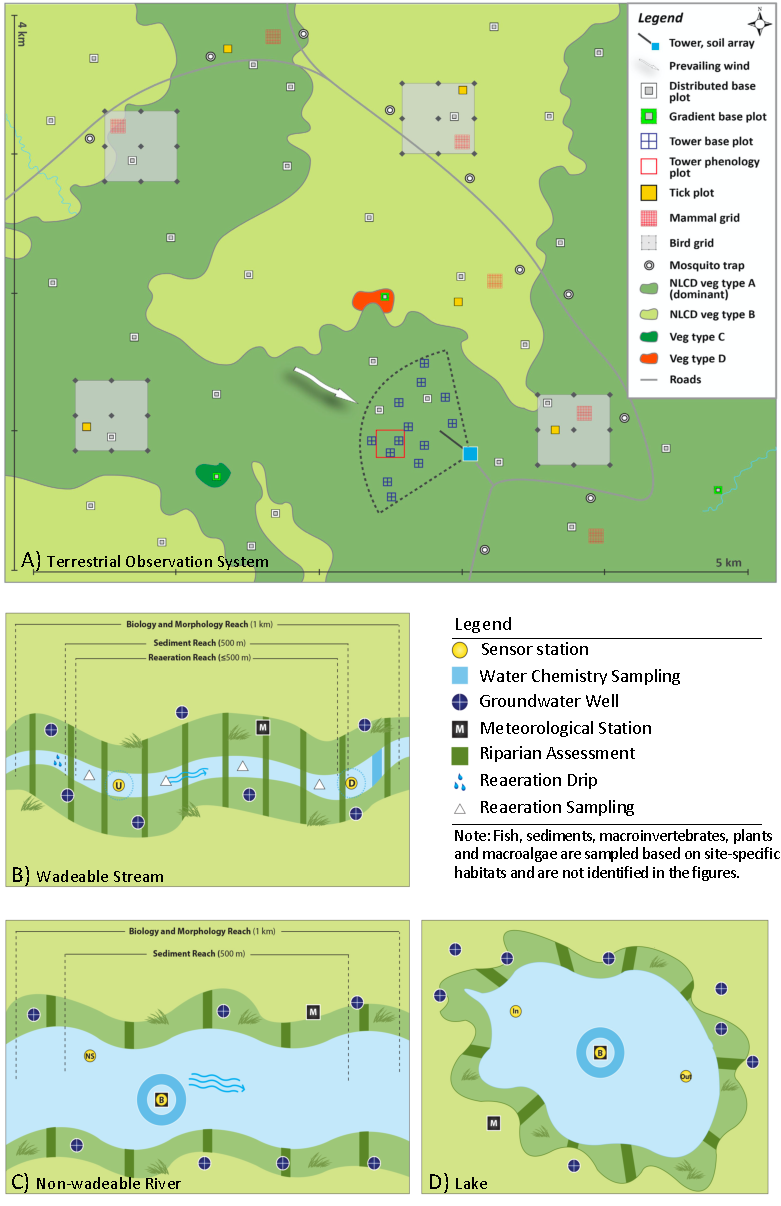
\includegraphics[width=0.95\linewidth]{/Users/dli/Github/neonDivData/manuscript/figures/fig_1} 

}

\caption{Generalized sampling schematics for Terrestrial Observation System (A) and Aquatic Observation System (B-D) plots. For Terrestrial Observation System (TOS) plots, Distributed, Tower, and Gradient plots, and locations of various sampling regimes, are presented via symbols. For Aquatic Observation System (AOS) plots, Wadeable stream, Non-wadeable stream, and Lake plots are shown in detail, with locations of sensors and different sampling regimes presented using symbols. Panel A was originally published by \protect\hyperlink{ref-thorpe2016introduction}{Thorpe et al.} (\protect\hyperlink{ref-thorpe2016introduction}{2016}).}\label{fig:Fig1Design}
\end{figure}

\hypertarget{terrestrial-organisms}{%
\subsection{Terrestrial Organisms}\label{terrestrial-organisms}}

\hypertarget{breeding-land-birds}{%
\subsubsection{Breeding Land Birds}\label{breeding-land-birds}}

\textbf{NEON Sampling Design} Landbirds are surveyed with point counts during the breeding season in each of the 47 terrestrial sites, co-located with distributed plots whenever possible (Fig. \ref{fig:Fig1Design}). Breeding landbirds are ``smaller birds (usually exclusive of raptors and upland game birds) not usually associated with aquatic habitats'' (\protect\hyperlink{ref-ralph1993handbook}{Ralph 1993}). At NEON sites, one sampling bout occurs per breeding season at large sites, and two sampling bouts occur at smaller sites. Point counts occur either within randomly distributed individual points or within bird grids at each site in representative (dominant) vegetation. At large NEON sites, 5-15 grids are sampled with nine point count locations each, where grid centers are co-located with distributed base plot centers, if possible. If small sites only allow five grids, a stratified random sample maintains 250 m minimum separation between point count locations and point counts occur at the southwest corner of the 5-25 distributed base plots.

The breeding season month, which defines the timing of sampling, varies somewhat by site but always occurs in the spring. Most species observed are diurnal and include both resident and migrant species. Early in the morning observers conduct point counts wherein the observer tracks each minute. Each point count contains species, sex, and distance to each bird (measured with a laser rangefinder except in the case of flyovers) seen or heard during a 6-minute period after a 2-minute acclimation period. To enable subsequent modeling of detectability, additional data collected during the point counts include: weather, distances from observers to birds, and the detection methods. The point count surveys for NEON were modified from the Integrated Monitoring in Bird Conservation Regions (IMBCR): Field protocol for spatially-balanced sampling of landbird populations (\protect\hyperlink{ref-pavlacky2017statistically}{Pavlacky Jr et al. 2017}).

To protect species of concern, their taxonomic IDs are `fuzzed.' This means the data are provided with a taxonomic identification at one higher taxonomic level than where the protection occurs. For example, if a threatened Black-capped vireo (\emph{Vireo atricapilla}) is recorded by a NEON technician, the taxonomic identification is fuzzed to Vireo in the data. Rare, threatened and endangered species are those listed as such by federal and/or state agencies.

\textbf{Data Wrangling Decisions} Bird point count data (`DP1.10003.001'), consist of a list of two associated data frames: \texttt{brd\_countdata} and \texttt{brd\_perpoint}). The former data frame contains information such as locations, species identities, and their counts. The second data frame contains additional location information such as latitude longitude coordinates and environmental conditions during the time of the observations. It is relatively straightforward to prepare the bird point count data for biodiversity research. We first combined both data frames into one and then removed columns that are likely not needed (e.g., laboratory names, publication dates, etc.).

The sampling protocol has evolved over time, so users are advised to check whether the \texttt{samplingProtocolVersion} fits their data requirements and subset as necessary. Zero counts could be excluded if desired by subsetting on the field \texttt{targetTaxaPresent} before proceeding. The field \texttt{taxonID} consists of the standard AOU 4-letter species code, although \texttt{taxonRank} refers to eight potential levels of identification (class, family, genus, species, speciesGroup, subfamily, and subspecies). Users can decide which level is appropriate, for example one might choose to exclude all unidentified birds (\texttt{taxonID\ =\ UNBI}), where no further details are available below the class level (Aves sp.).

\hypertarget{ground-beetles-and-herp-bycatch}{%
\subsubsection{Ground Beetles and Herp Bycatch}\label{ground-beetles-and-herp-bycatch}}

\textbf{NEON Sampling Design} Each site is sampled with pitfall traps, with 10 separate distributed plots at each site and four pitfall traps at each plot initially - placed in the ground along the cardinal directions of the distributed plot boundary. This equates to a total of 40 pitfall traps per site. In 2018, sampling was reduced via the elimination of the North pitfall trap in each plot, resulting in 30 traps per site. Sampling begins when the temperature has been \textgreater{} 4°C for 10 days in the spring and ends when temperatures dip below this threshold in the fall. Sampling occurs biweekly throughout the sampling season with no single trap being sampled more frequently than every 12 days. After collection, the samples are separated into carabid species and bycatch, with bycatch archived at either the trap (vertebrate) or plot (invertebrate) level. Carabid samples and vertebrate bycatch are sorted and identified by NEON technicians, after which a subset of carabid individuals are sent to be pinned and re-identified by an expert taxonomist. More details can be found in \protect\hyperlink{ref-hoekman2017design}{Hoekman et al.} (\protect\hyperlink{ref-hoekman2017design}{2017}).

Pitfall traps and sampling methods are designed by NEON to reduce vertebrate bycatch \protect\hyperlink{ref-hoekman2017design}{Hoekman et al.} (\protect\hyperlink{ref-hoekman2017design}{2017}). The pitfall cup is medium in size with a low clearance cover installed over the trap entrance to minimize large vertebrate bycatch. When a live vertebrate with the ability to move on its own volition is found in a trap, the animal is released. Live but morbund vertebrates are euthanized and collected along with deceased vertebrates. When 15 or more individuals of a vertebrate species are collected, cumulatively, within a single plot, NEON may initiatie localized mitigation measures such as temporarily deactivating traps and removing all traps from the site for the remainder of the season. Thus, while herpetofaunal (herp) bycatch is present in many pitfall samples, due to these active efforts to reduce vertebrate bycatch, it is unclear how well these pitfall traps capture herp community structure and diversity and users of the herp bycatch data we wrangle and provide here should be aware of these limitations.

\textbf{Data Wrangling Decisions} Beetle samples are identified at multiple levels of expertise. Beetles are first identified by the sorting technician and then the pinning technician. Identifications of more difficult specimens are additionally verified by an expert taxonomist. Whenever available, expert identification is used for a sample. For example, if taxonomic delineation between NEON staff and multiple expert taxonomist identifications do not agree, then the consensus expert taxonomist delineation is recorded in the data portal. However, these differences in taxonomic expertise do not seem to cause systematic biases in estimating species richness across sites, but non-expert taxonomists are more likely to misidentify non-native carabid species (\protect\hyperlink{ref-egli2020taxonomic}{Egli et al. 2020}).

Beetle abundances are recorded on the sorted sample, by NEON technicians, and are not preserved across the different levels of identification. For example, a sample of 15 individuals identified during the sorting phase may be passed to a pinning technician, who then identifies five different species within that sample. The pinning technician does not back annotate the sorted sample to identify which individuals are which species, or go through and re-identify the rest of the individuals in the sample. Without this, we have assumed that all individuals in the sorted sample that were not positively identified by an expert were correctly identified in the original sample by NEON technicians. Hence, the abundance for a newly identified species is one, and the abundance for the originally identified species for the sample is the original abundance minus the individuals expertly identified as a different species.

Sometimes there are more individuals identified by pinning technicians or experts than were counted in the original sorted sample, so the count has been updated in the dataset. There are also a few cases where an especially difficult identification was sent to multiple expert taxonomists and they did not agree on a final taxon, these individuals were excluded from the data set at the recommendation of NEON staff.

Prior to 2018, \texttt{trappingDays} values were not included for many sites. Missing entries were calculated as the range from \texttt{setDate} through \texttt{collectDate} for each trap. We also account for a few plots for which \texttt{setDate} was not updated based on a previous collection event in the \texttt{trappingDays} calculations. To facilitate easy manipulation of data within and across bouts a new \texttt{boutID} field was created to identify all trap collection events at a site in a bout. The original \texttt{EventID} field is intended to identify a bout, but has a number of issues that necessitates creation of a new ID. First, \texttt{EventID} does not correspond to a single collection date but rather all collections in a week. This is appropriate for the small number of instances when collections for a bout happen over multiple consecutive days (\textasciitilde5\% of bouts), but prevents analysis of bout patterns at the temporal scale of a weekday. The data here were updated so all entries for a bout correspond to the date (i.e., \texttt{collectDate}) on which the majority of traps are collected to maintain the weekday-level resolution with as high of fidelity as possible, while allowing for easy aggregation within bouts and \texttt{collectDate}'s. Second, there were a few instances in which plots within a site were set and collected on the same day, but have different \texttt{EventID}'s. These instances were all considered a single bout by our new \texttt{boutID}, which is a unique combination of \texttt{setDate}, \texttt{collectDate}, and \texttt{siteID}.

Herpetofaunal bycatch (amphibian and reptile) in pitfall traps are counted identified to species or the lowest taxonomic level possible within 24 h of recovery from the field. To process the herp bycatch NEON data we cleaned \texttt{trappingDays} and the other variables and added \texttt{boutID} as described above for beetles. The variable \texttt{sampleType} in the \texttt{bet\_sorting} table provides the type of animal caught in a pitfall trap as one of five types: \texttt{carabid}, \texttt{vert\ bycatch\ herp}, \texttt{other\ carabid}, \texttt{invert\ bycatch} and \texttt{vert\ bycatch\ mam}. We filtered the beetle data described above to only include the \texttt{carabid} and \texttt{other\ carabid} types. For herps, we only kept the \texttt{sampleType} of \texttt{vert\ bycatch\ herp}.

\hypertarget{mosquitos}{%
\subsubsection{Mosquitos}\label{mosquitos}}

\textbf{NEON Sampling Design} Mosquito specimens are collected at 47 terrestrial sites across all NEON domains. Traps are distributed throughout the site according to a stratified-random spatial design used for all Terrestrial Observation System sampling, and are typically located within 30m of a road to facilitate expedient sampling. NEON collects mosquito specimens using the Center for Disease Control (CDC) CO\textsubscript{2} light traps. These traps have been used by other public health and mosquito-control agencies for a half-century, which allows NEON mosquito data to be used across field sites and in combination with existing long-term data sets. A CDC CO\textsubscript{2} light trap consists of a cylindrical insulated cooler that contains dry ice, a plastic rain cover attached to a battery powered light/fan assembly, and a mesh collection cup. During deployment, the dry ice sublimates and releases CO\textsubscript{2}. Mosquitoes attracted to the CO\textsubscript{2} bait are sucked into the mesh collection cup by the battery-powered fan, where they remain alive until trap collection.

Mosquito monitoring is divided into field season and off-season sampling. Off-season sampling takes place weekly at core sites, and begins after three consecutive zero-catch field sampling bouts at the core site. The goal of off-season sampling is to rapidly determine when the next field season should begin and to provide mosquito phenology data throughout the lifetime of the observatory. During the off season, overnight sampling occurs weekly at three dedicated mosquito plots spread throughout the terrestrial core sites for each domain while temperatures are \textgreater10 °C. Traps are deployed at dusk and checked the following dawn. Field season sampling begins when the first mosquito is detected during off season sampling.

Technicians collect samples every two weeks at core terrestrial sites and every four weeks at relocatable terrestrial sites. Sampling occurs at 10 dedicated mosquito plots at each site over a 24-hour period, or one sampling bout. During the sampling bout, traps are serviced twice and yield one night-active sample, taken at dawn or about eight hours after the trap is set, and one day-active sample, taken at dusk or \textasciitilde16 hours after the trap is set. Thus, a 24-hour sampling bout yields 20 ``samples'' from 10 traps.

Following field collection, NEON's field ecologists process, pack up and ship the samples to an external lab where mosquitoes are identified to species and sex (when possible). A subset of identified mosquitoes are tested for infection by pathogens to quantify the presence/absence and prevalence of various arboviruses. Some mosquitoes are set aside for DNA barcode analysis as well as long-term archiving. Particularly rare or difficult to identify mosquito specimens are prioritized for DNA barcoding. More details can be found in \protect\hyperlink{ref-hoekman2016design}{Hoekman et al.} (\protect\hyperlink{ref-hoekman2016design}{2016}).

\textbf{Data Wrangling Decisions} \textbf{Data Wrangling Decisions} Mosquito data are mainly stored in four data frames: trapping data (\texttt{mos\_trapping}), sorting data (\texttt{mos\_sorting}), archiving data (\texttt{mos\_archivepooling}), and expert taxonomist processed data (\texttt{mos\_expertTaxonomistIDProcessed}). We first removed rows (records) with missing important information about location, collection date, and sample or subsample ID for all data frames. We then merged all four data frames into one while checked carefully that they are merged correctly. In the merged data frame, we only kept records for target taxa (i.e., \texttt{targetTaxaPresent\ ==\ "Y"}) and no known compromised sampling condition (i.e., \texttt{sampleCondition\ ==\ "No\ known\ compromise"}). We further removed a small number of records with species identified only to the family level; all remaining records were identified at least at the genus level. We estimated the total individual count for each species within a trap as \texttt{individualCount\ *\ (totalWeight\ /\ subsampleWeight)}. We then removed columns that likely will not be used for calculating biodiversity values.

\hypertarget{small-mammals}{%
\subsubsection{Small Mammals}\label{small-mammals}}

\textbf{NEON Sampling Design} NEON defines small mammals based on taxonomic, behavioral, dietary, and size constraints, and includes any rodent that is (1) nonvolant; (2) nocturnally active; (3) forages predominantly aboveground; and (4) has a mass \textgreater5 grams, but \textless{} about 500-600 grams. In North America, this includes cricetids, heteromyids, small sciurids, and introduced murids, but excludes shrews, large squirrels, rabbits, or weasels, although individuals of these species may be incidentally captured. Small mammals are collected at NEON sites using Sherman traps, identified to species in the field, marked with a unique tag, and released. Multiple 90 m x 90 m trapping grids are set up in each terrestrial field site within the dominant vegetation type. Each 90 m x 90 m trapping grid contains 100 traps placed in a pattern with 10 rows and 10 columns set 10 m apart. Three 90 m x 90 m grids per site are designated pathogen grids and the remainder are designated diversity grids. Small mammal sampling occurs in bouts, with a bout comprised of three consecutive (or nearly consecutive) nights of trapping, and is based on the lunar calendar, with timing of sampling constrained to occur within 10 days before or after the new moon. The number of bouts per year is determined by site type, and most sites contain six bouts per year.

\textbf{Data Wrangling Decisions} In the data presented, records are stratified by NEON site, year, month, and day and represent data from both the diversity and pathogen sampling grids. Capture records were removed if they were not identified to genus or species (e.g., if the species name was denoted as `either/or' or as family name), if they represented dead animals (fate = `dead') or escaped animals (fate = `escaped'), or bycatch (fate = `nontarget,' i.e., non-target species). Records for recaptured individuals were also removed. However, we kept empty traps as they contain information about sampling efforts, which can be useful for some studies.

\hypertarget{soil-microbes}{%
\subsubsection{Soil Microbes}\label{soil-microbes}}

\textbf{NEON Sampling Design} Soil samples are collected at ten 40 x 40 m2 NEON plots per site. Four plots are within the tower airshed (tower plots), and six plots are distributed across the landscape (gradient plots). At each sampling time point, soils are sampled from three of the four subplots, and one sample collected from a randomly-generated XY coordinate location within each subplot. At each sampling location, soils are taken at the surface horizon most years, but from both organic and mineral horizons every five years during coordinated microbe/biogeochemistry bouts. Most sites, except for the boreal/arctic sites, are sampled three times a year, once at peak vegetation greenness and two other times bracketing that period. This results in \textasciitilde10 plots * 3 locations * 1 or 2 horizons * 3 periods = 90 - 180 soil samples per site per year for most sites. Samples for microbial biomass, composition, and metagenomics are stored on dry ice and shipped to an external lab (variable depending on year) for downstream processing.

\textbf{Data Wrangling Decisions} Unlike other NEON biodiversity data, the soil microbial datasets require significant pre-processing to go from raw sequence data to a community matrix, and the exact bioinformatics methods will vary depending on use case. Briefly, major decisions during this process will depend on whether users are working with fungal (ITS) or bacterial (16S) data, if the goal is to maximize read quality and taxonomic resolution vs.~number of reads retained through the quality filter process, and whether to remove or retain reverse complement reads for a merged sequence. The full description of a suggested bioinformatics pipeline, how to run sensitivity analyses on user-defined parameters, accompanying code, and vignettes are described in Qin \emph{et al} in this issue. At the end of the suggested bioinformatics pipeline, users will have a phyloseq object, which is a commonly-used format for sequence-based analysis software. The phyloseq object will contain a table of ASV (amplicon sequence variant) sequences, a table of taxonomic assignments, and soil chemical and physical data associated with the same sample locations and sampling bouts.

\hypertarget{terrestrial-plants}{%
\subsubsection{Terrestrial Plants}\label{terrestrial-plants}}

\textbf{NEON Sampling Design} NEON plant diversity plots are sampled during one or two bouts per year, and are 400 m x 400 m in size. Sampling is done using a nested design, where the entire plot is first subdivided into 4 100 m x 100 m subplots. For each subplot, one or more 1 m x 1 m nested subplots are then sampled; species coverages within the 1 m\textsuperscript{2} area are estimated visually. Next presence/absence of plants is recorded in one or more 10 m x 10 m subplots, inside of which the finer resolution subplots are located. Finally, the 100 m x 100 m subplot is sampled for presence/absence of plants. At the 10 m by 10 m and 100 m by 100 m scales, only presence and absence of plants were recorded. Each species is recorded only once during sampling, such that an observation of a species at a finer-resolution subplot prevents it from being recorded again if it is encountered in a coarser-resolution subplot. A full dataset for each NEON plant diversity plot was generated by combining all data from all subplots within the 400 m x 400 m boundary, and removing duplicates (which may occur across the 100 m x 100 m subdivisions). More details about the sampling design can be found in \protect\hyperlink{ref-barnett2019plant}{Barnett et al.} (\protect\hyperlink{ref-barnett2019plant}{2019}).

NEON manages plant taxonomic entries with a master taxonomy list that is based on the community standard, where possible. Using this list, synonyms for a given species are converted to the currently used name. The master taxonomy for plants is the USDA PLANTS Database (USDA, NRCS. 2014. \url{https://plants.usda.gov}), and the portions of this database included in the NEON plant master taxonomy list are those pertaining to native and naturalized plants present within the NEON sampling area. A sublist for each NEON domain includes those species with ranges that overlap the domain as well as nativity designations - introduced or native - in that part of the range. If a species is reported at a location outside of its known range, and the record proves reliable, the master taxonomy list is updated to reflect the distribution change. For more on the NEON plant master taxonomy list see NEON.DOC.014042 (\url{https://data.neonscience.org/api/v0/documents/NEON.DOC.014042vK}).

\textbf{Data Wrangling Decisions} Sampling at the 1 m x 1 m scale also includes observations of abiotic and non-target species ground cover (i.e., soil, water, downed wood), so we removed records with \texttt{divDataType} as ``otherVariables.'' We also removed records whose \texttt{targetTaxaPresent} is \texttt{N} (i.e., a non-target species). Additionally, for all spatial resolutions (i.e., 1 m x 1 m, 10 m x 10 m, and 100 m x 100 m data), any record lacking information critical for combining data within a plot and for a given sampling bout (i.e., \texttt{plotID}, \texttt{subplotID}, \texttt{boutNumber}, \texttt{endDate}, or \texttt{taxonID}) was dropped from the dataset. Furthermore, records without a definitive genus or species level \texttt{taxonID} (i.e., those representing unidentified morphospecies) were not included. To combine data from different spatial resolutions into one data frame, we created a pivot column entitled \texttt{sample\_area\_m2} (with possible values of 1, 100, and 10000). Because of the nested sampling design of the plant data, to capture all records within a subplot at 10 m by 10 m scale, we incorporated all data from both the 1 m by 1 m and 10 m by 10 m scales for that subplot. Similarly, to obtain all records within a subplot at the 100 m by 100 m scale, we included all data from that subplot. Species abundance information was only recorded as area coverage within 1 m by 1 m subplots; however, users may use the frequency of a species across subplots within a plot or plots within a site as a proxy of its abundance if needed.

\hypertarget{ticks-and-tick-pathogens}{%
\subsubsection{Ticks and Tick Pathogens}\label{ticks-and-tick-pathogens}}

\textbf{NEON Sampling Design} Tick sampling occurs in six distributed plots at each site, which are randomly chosen in proportion to NLCD land cover class. Sampling begins on a low intensity schedule with one sampling bout every six weeks. Once \textgreater5 ticks of any life stage have been collected within the last year at that site, sampling switches to a high intensity schedule with one bout every three weeks. A site remains on the high intensity schedule until \textless5 ticks are collected within a year, then it reverts back to the low intensity schedule. High intensity sampling reoccurs when \textgreater5 ticks are collected within a year. Onset of sampling coincides with phenological milestones at each site, beginning within two weeks of the onset of green-up and ending within two weeks of vegetation senescence. Sampling bouts are only initiated if the high temperature on the two consecutive days prior to planned sampling was \textgreater0°C.

Ticks are sampled by walking the perimeter of a 40 m x 40 m plot using a 1 m x 1 m drag cloth. Ideally, 160 meters are sampled (shortest straight line distance between corners), but the cloth can be dragged around obstacles if a straight line is not possible. Acceptable total sampling area is between 80-180 meters. The cloth can also be flagged over vegetation when the cloth cannot be dragged across it. Ticks are collected from the cloth and technicians' clothing at appropriate intervals depending on vegetation density and at every corner of the plot and are immediately transferred to a vial containing RNA stabilization solution.

Ticks are sent to the US National Tick Collection at Georgia Southern University for identification to species, life stage, and sex. A subset of nymphal ticks are sent to the Laboratory of Medical Zoology at the University of Massachusetts Amherst for pathogen testing. \emph{Ixodes scapularis} are tested for \emph{Anaplasma phagocytophilum}, \emph{Babesia microti}, \emph{Borrelia burgdorferi} sensu lato, \emph{Borrelia miyamotoi}, \emph{Borrelia mayonii}, other \emph{Borrelia} species (\emph{Borrelia} sp.), and a \emph{Ehrlichia} muris-like agent (\protect\hyperlink{ref-pritt2017proposal}{Pritt et al. 2017}). \emph{Amblyomma americanum} was tested for \emph{Anaplasma phagocytophilum}, \emph{Borrelia lonestari} (and other undefined \emph{Borrelia} species), \emph{Ehrlichia chaffeensis}, \emph{Ehrlichia ewingii}, \emph{Francisella tularensis}, and \emph{Rickettsia rickettsii}.

\textbf{Data Wrangling Decisions} We downloaded the tick drag and taxonomic identification data (DP1.10093.001; \texttt{tck\_taxonomyProcessed} hereafter referred to as `taxonomy data'; \texttt{tck\_fielddata} hereafter referred to as `field data') via the NEON API. We note that end users should be aware of some issues related to taxonomic ID. Counts assigned to higher taxonomic levels (e.g., at the order level \emph{Ixodida}; IXOSP2) are not the sum of lower levels; rather they represent the counts of individuals that could not reliably be assigned to a lower taxonomic unit. Some identifications (e.g., IXOSPP) represent potentially mixed samples with more than one species present. Users should exercise caution when computing metrics like richness from these data. Finally, we assigned those samples that were not identified in the lab to the highest taxonomic level (order \emph{Ixodida}; IXOSP2). However, users could make an informed decision to assign these ticks to the most probable group if a subset of individuals from the same sample were assigned to a lower taxonomy.

First, in the field data, we removed samples that had sampling issues and samples with no count data, which mostly consisted of 2019 data that had not been processed. Next, we removed field samples that did not have corresponding taxonomic information. Conversely, we removed taxonomy samples that did not have corresponding field information, many of which were legacy samples where larvae were not counted. We retained these records where no ticks were found in a sampling bout. In the taxonomy data, we removed samples that did not have an ``OK'' sample condition.

We left-joined the field data to the taxonomy data to preserve zeros in the count data. To merge the two datasets, we combined `male' or `female' into one `adult' class. Next, we reconciled differences in counts between the two datasets, generally placing greater confidence in the counts from the taxonomy lab (note that beginning in 2019, counts are only taken by taxonomists, so reconciling field and lab counts will no longer be necessary). If the lab determined no ticks were present in the sample (e.g., ticks were mis-identified in the field), we corrected the field data to match the taxonomy data. When there were discrepancies between the identified life-stages but not the total counts of ticks, we retained the counts from the lab. Larvae were not always identified or counted in the lab, or if they were, were only counted up to a limit. If there were more larvae in the field than in the lab (7\% of samples), we assigned the remaining unidentified larvae to the order level (IXOSP2). Similarly, in some cases the lab only identified ticks up to a certain invoicing limit, usually 500 individuals. In these cases (2\% of samples) we assigned remaining unidentified ticks to the order level.

In cases where counts were off by only a few individuals (3\% of samples), we attributed these to miscounts in the field or ticks lost in transit and trusted the taxonomy counts. In cases where one to two ticks in the field data were missing but the discrepancy was \textgreater10\% of the total count, we assigned those missing ticks to the order level in an adult-specific column. In cases with larger discrepancies without an obvious remark describing it (0.1\% of cases), we removed the sample from the dataset, making sure that these cases were \textless1\% of the size of the total dataset. We note that the majority of samples (\textasciitilde85\%) had no discrepancies between the lab or field, therefore this process could be ignored by users for whom analyses are not sensitive to exact counts.

For tick pathogens, we downloaded tick pathogen data (DP1.10092.001; \texttt{tck\_pathogen} hereafter referred to as `pathogen data'; \texttt{tck\_pathogenqa} hereafter referred to as `quality data') via the NEON API. First, we removed any samples that had flagged quality checks from the quality data and removed any samples that did not have a positive DNA quality check from the pathogen data. Although the original online protocol aimed to test 130 ticks per site per year from multiple tick species, the final sampling decision was to extensively and thoroughly test IXOSCA and AMBAME species only. \emph{Borrelia burgdorferi} and \emph{Borrelia burgdorferi sensu lato} tests were merged, since the former was an incomplete pathogen name and likely referred to \emph{B. burgdorferi sensu lato} as opposed to \emph{sensu stricto} (\protect\hyperlink{ref-rudenko2011updates}{Rudenko et al. 2011}). Tick host species was not included in the original data sheet, but we manually added these to the cleaned data sheets by extracting tick species from subsampleID names.

\hypertarget{aquatic-organisms}{%
\subsection{Aquatic Organisms}\label{aquatic-organisms}}

\hypertarget{aquatic-macroinvertebrates}{%
\subsubsection{Aquatic macroinvertebrates}\label{aquatic-macroinvertebrates}}

\textbf{NEON Sampling Design} Aquatic macroinvertebrate sampling occurs three times/year at wadeable stream, river, and lake sites from spring through fall. Samplers vary by habitat and include Surber, Hess, hand corer, modified kicknet, D-frame sweep, and petite ponar samplers. Lake sampling occurs with a petite ponar near buoy, inlet, and outlet sensors, and D-frame sweeps in littoral zones. Riverine sample collections in deep waters or near buoys are made with a petite ponar, and in littoral areas are made with a D-frame sweep or large-woody debris sampler. In the field, samples are preserved in pure ethanol, but later in the domain support facility, glycerol is added to prevent the samples from becoming brittle. Samples are shipped from the domain facility to a taxonomy lab for sorting and identification to lowest possible taxon (e.g., genus or species) and counts of each taxon per size are made to the nearest mm.

\textbf{Data Wrangling Decisions} We downloaded the aquatic macroinvertebrate taxonomic identification, data quality, and related field data (DP1.20120.001; Macroinvertebrate collection) using the NEON API. Aquatic macroinvertebrates are subsampled and identified to the lowest practical taxonomic level, typically genus, by expert taxonomists in the \texttt{inv\_taxonomyProcessed} table, measured to the nearest mm size class, and counted. Taxonomic naming has been standardized in the \texttt{inv\_taxonomyProcessed} files, according to NEON's master taxonomy (\url{https://data.neonscience.org/taxonomic-lists}), removing any synonyms. We calculated macroinvertebrate density by dividing \texttt{estimatedTotalCount} (which includes the corrections for subsampling in the taxonomy lab) by \texttt{benthicArea} from the \texttt{inv\_fieldData} table to return count per square meter of stream/lake/river bottom.

\hypertarget{microalgae-periphyton-and-phytoplankton}{%
\subsubsection{MicroAlgae (Periphyton and Phytoplankton)}\label{microalgae-periphyton-and-phytoplankton}}

\textbf{NEON Sampling Design} Algal sampling methods vary by system (i.e., wadeable streams, rivers, lakes) and are sampled three times per year (i.e., spring, summer, and fall). In wadeable streams, which have variable habitats (e.g., riffles, runs, pools, step pools), five periphyton samples are collected in the dominant habitat type and three in the second most dominant habitat type over a 1km reach. No two samples should come from the sample habitat unit (i.e., same riffle).

Periphyton samples are collected from natural surface substrata with the specific collection method and sampler type dependent on the substrate type (i.e., cobble vs.~silt vs.~woody debris) (see \protect\hyperlink{ref-moulton2002revised}{Moulton II et al. 2002} for detailed methods). Periphyton is also collected from lakes and rivers from five areas in the littoral zone (i.e., shoreline) with the most dominant substratum type selected. In rivers, phytoplankton are sampled near the sensor buoy and at two other deep-water points in the main channel, using a Kemmerer sampler. For lakes, phytoplankton are collected by the central sensor buoy as well as at the inlet and outlet sensor sensors, using a Kemmerer sampler. For stratified lakes and non-wadeable streams, the phytoplankton sample is a composite from one surface sample, one sample from the metalimnion (i.e., middle layer), and one sample from the bottom of the euphotic zone. For non-stratified lakes and non-wadeable streams, the phytoplankton sample is a composite from one surface sample, one sample just above the bottom of the euphotic zone, and if the euphotic zone is \textgreater{} 5 m, then one mid-euphotic zone sample.

Samples are processed at the domain support facility and separated into subsamples for taxonomic analysis or for biomass measurements. Aliquots shipped to an external facility for taxonomic determination are preserved in glutaraldehyde or Lugol's iodine. Aliquots for biomass measurements are filtered onto glass-fiber filters and processed for ash-free dry mass.

\textbf{Data Wrangling Decisions} We downloaded the algae taxonomic identification, biomass and related field data (DP1.20166.001; `Periphyton, Seston and Phytoplankton Collection' hereafter referred to as \texttt{alg\_tax\_long}, \texttt{alg\_biomass} and \texttt{alg\_field\_data}) via the NEON API. Algae within samples are identified to the lowest possible taxonomic resolution, usually species, by contracting laboratory taxonomists. Some specimens can only be identified to the genus or even class level, depending on the condition of the specimen. Ten percent of all samples are checked by a second taxonomist and are noted in the \texttt{qcTaxonomyStatus}. Taxonomic naming has been standardized in the \texttt{alg\_tax\_long} files, according to NEON's master taxonomy, removing nomenclatural synonyms. Abundance and cell/colony counts are determined for each taxon of each sample with counts of cells or colonies that are either corrected for sample volume or not (as indicated by algalParameterUnit = `cellsperBottle').

We corrected sample units of \texttt{cellsperBottle} to density. First, we summed the preservative volume and the lab's recorded sample volume for each sample (from the \texttt{alg\_biomass} file) and combined that with the \texttt{alg\_tax\_long} file using \texttt{sampleID} as a common identifier. Many samples in the \texttt{alg\_tax\_long} file were missing data in the \texttt{perBottleSampleVolume} field, so a new field called \texttt{perBSVol} was created using NEON domain lab sample volumes. With this updated file, we combined it with \texttt{alg\_field\_data} to have the related field conditions, including benthic area sampled for each sample. \texttt{parentSampleID} was used for \texttt{alg\_field\_data} to join to the \texttt{alg\_biomass} file's \texttt{sampleID} as \texttt{alg\_field\_data} only has \texttt{parentSampleID}. We then calculated cells per milliliter for the uncorrected taxon of each sample, dividing \texttt{algalParameterValue} by the updated sample volume \texttt{perBSVol}. Benthic sample results are expressed in terms of area (multiplied by the field sample volume, divided by benthic area sampled), in square meters. The final abundance units are either cells/mL (phytoplankton and seston samples) or cells/m\textsuperscript{2} for benthic samples.

The \texttt{sampleIDs} are child records of each \texttt{parentSampleID} that will be collected as long as sampling is not impeded (i.e., ice covered or dry). In the \texttt{alg\_biomass} file, there should be only a single entry for each \texttt{parentSampleID}, \texttt{sampleID}, and \texttt{analysisType}. Most often, there were two \texttt{sampleID}'s per \texttt{parentSampleID} with one for ash free-dried mass (ADFM) and taxonomy (analysis types). For the creation of the observation table with standardized counts, we used only records from the \texttt{alg\_biomass} file with the \texttt{analysisType} of taxonomy. In \texttt{alg\_tax\_long}, there are multiple entries for each \texttt{sampleID} for each taxon by \texttt{scientificName} and \texttt{algalParameter}.

\hypertarget{fish}{%
\subsubsection{Fish}\label{fish}}

\textbf{NEON Sampling Design} Fish sampling is carried out across 19 NEON-designated ecoregions including both lotic (23 stream habitats) and lentic (five lake habitats) habitats. Each site is surveyed with two bouts per year, during the spring and fall, with a combination of random and fixed sampling areas (i.e., segments in lakes; reaches in streams) to capture spatial and temporal heterogeneity of aquatic habitats. Each sampling bout is completed within five days with a minimum two-week gap in between two successive sampling bouts. The initial sampling date is determined using site-specific historical data on ice melting, water temperature (or accumulated degree days), and riparian peak greenness.

At each lake, 10 sector-shaped segments are established, wherein each segment ranges from the riparian zone into the lake center, therefore effectively capturing both nearshore and offshore habitats. Three of the 10 segments are fixed, which encompasses habitat features most representative of the entire lake, and are surveyed twice a year with a backpack electrofisher using a three-pass electrofishing depletion approach (\protect\hyperlink{ref-moulton2002revised}{Moulton II et al. 2002}, \protect\hyperlink{ref-peck2006environmental}{Peck et al. 2006}). All three passes in a fixed sampling segment or reach are completed on the same day, with a minimum gap of 30-minutes between successive passes. Additionally, a fyke net and a gill net are deployed at each fixed segment (\protect\hyperlink{ref-baker1997environmental}{Baker et al. 1997}). The remaining random segments are sampled on a rotation design with a single electrofishing pass, one mini-fyke net, and one gill net where three segments are surveyed twice a year.

In each stream site, a maximum of 10 non-overlapping reaches (each reach 70-130m in length) are designated within a 1km stream length, with six of those reaches sampled during any given sampling bout. The 10 reaches include three fixed reaches that are consistently sampled and seven random reaches that are sampled on rotation. The three fixed reaches encompass all representative habitats found within a 1-km-stretch and are surveyed twice a year (once in each bout) using a three-pass electrofishing depletion approach (\protect\hyperlink{ref-moulton2002revised}{Moulton II et al. 2002}, \protect\hyperlink{ref-peck2006environmental}{Peck et al. 2006}). The random reaches are surveyed on rotation via a single-pass depletion approach; three random reaches are sampled twice a year (once in each bout), while another three random reaches are sampled in the subsequent year. Electrofishing at streams is done during daytime. At lake sites, electrofishing is started and ceases 30-minutes after and before sunset and sunrise, respectively, with a maximum of five passes per sampling bout. Gill nets are deployed for 1-2 hrs either in the morning or early afternoon, while fyke nets are positioned before sunset and recovered after sunrise on the following day. Precise start and end times for both electrofishing and net deployments are documented.

In all surveys, captured fish are identified to the lowest practical taxonomic level, and morphometrics (i.e., body mass and body length) are recorded before releasing. Relative abundance for each fish taxon is also recorded by direct enumeration or estimation (i.e., by scooping and counting the total number of specimens in one dip net and then multiplying the total number of scoops of captured fish by the counts from the first scoop).

\textbf{Data Wrangling Decisions} Fish sampled via both electrofishing and trapping are identified at variable taxonomic resolutions (up to subspecies level) in the field. Most identifications are made to the species or genus level by a single field technician for a given bout per site. Sampled fish are identified, photographed, measured, weighed, and then released back to the site of capture. If field technicians are unable to identify to the species level, such specimens are (1) either identified to the finest possible taxonomic resolution or 2) assigned a morphospecies with a coarse-resolution identification. The standard sources consulted for identification and a qualifier for identification validity are also documented in the \texttt{fsh\_perFish} table. The column \texttt{bulkFishCount} of the \texttt{fsh\_bulkCount} table records relative abundance for each species or the alternative next possible taxon level (specified in the column \texttt{scientificName}). Local fish taxonomists in each NEON domain identify the morphospecies and species with uncertain taxonomic identities.

Fish data (taxonomic identification and relative abundance) are recorded per each sampling reach in streams or segment in lakes in each bout. The column \texttt{eventID} uniquely identifies the sampling date of the year, the specific site within the domain, a reach/segment identifier, the pass number (i.e., number of electrofishing passes or number of net deployment efforts), and the survey method. A \texttt{reachID} column is also provided that uniquely identifies surveys done per stream reach or lake segment. The \texttt{reachID} is nested within the \texttt{eventID} as well. We used \texttt{eventID} as a nominal variable to uniquely identify different sampling events and to join different, stacked fish data files as described below.

We downloaded all fish data (i.e., \texttt{fsh\_perPass}, \texttt{fsh\_fieldData}, \texttt{fsh\_bulkCount}, \texttt{fsh\_perFish}), including the complete taxon table for fish, for both stream and lake sites surveyed via the NEON API. We joined the \texttt{fsh\_perPass}, \texttt{fsh\_fieldData}, and \texttt{fsh\_bulkCount} datasets to produce a table with bulk-processed data that merged \texttt{fsh\_perPass}, \texttt{fsh\_fieldData}, and \texttt{fsh\_perFish} to concatenate individual-level data. Finally both individual-level and bulk-processed datasets were appended into a single table. For each finer-resolution taxon in the individual-level dataset, we considered the relative abundance as one since each row represented a single individual fish. Whenever possible, we substituted missing data by cross-referencing other data columns, omitted completely redundant data columns, and retained records with genus- and species-level taxonomic resolution. For the appended dataset, we also calculated the relative abundance for each species per sampling reach or segment at a given site. To calculate species-specific catch per unit effort (CPUE), we normalized the relative abundance by either average electrofishing time (i.e., \texttt{efTime}, \texttt{efTime2}) or trap deployment time (i.e., the difference between \texttt{netEndTime} and \texttt{netSetTime}). In this case, we assumed that size of the traps used, water depths, number of netters used, and the reach lengths (a significant proportion of bouts had reach lengths missing) to be comparable across different sampling reaches and segments.

\hypertarget{zooplankton}{%
\subsubsection{Zooplankton}\label{zooplankton}}

\textbf{NEON Sampling Design} Zooplankton samples are collected at 7 NEON lake sites across 4 domains. Zooplankton samples are collected at the buoy sensor set (deepest location in the lake) and at the two nearshore sensor sets using a vertical tow net for locations deeper than 4 m, and a Schindler trap for location shallower than 4 m. This results in 3 samples collected per sampling day. Samples are preserved with ethanol in the field and shipped from the domain facility to a taxonomy lab for sorting and identification to lowest possible taxon (e.g., genus or species) and counts of each taxon per size are made to the nearest mm.

\textbf{Data Wrangling Decisions} We downloaded the zooplankton taxonomic identification and related field data (DP1.20219.001). Zooplankton in NEON samples are identified at contracting labs to the lowest possible taxonomic resolution, usually genus, however some specimens can only be identified to the family (or even class) level, depending on the condition of the specimen. Ten percent of all samples are checked by two taxonomists and are noted in the \texttt{qcTaxonomyStatus}. The taxonomic naming has been standardized in the \texttt{zoo\_taxonomyProcessed} table, according to NEON's master taxonomy, removing any synonyms. Density was calculated using \texttt{adjCountPerBottle} and \texttt{towsTrapsVolume} to correct count data to ``count per liter.''

\hypertarget{results-or-how-to-get-and-use-tidy-neon-organismal-data}{%
\section{Results (or how to get and use tidy NEON organismal data)}\label{results-or-how-to-get-and-use-tidy-neon-organismal-data}}

All cleaned data products can be obtained from the R package \texttt{neonDivData}, which can be installed from Github. Installation instructions can be found on the Github webpage (\url{https://github.com/daijiang/neonDivData}). Table \ref{tab:dataSummary} shows the brief summary of all data products. To get a specific data product, we can just call the objects in the \texttt{data\_product} column in Table \ref{tab:dataSummary}. Such data products include cleaned (and standardized if needed) occurrence data for the taxonomic groups covered and are equivalent to the ``observation'' table of the ecocomDP data format. If environmental information and species measurements were provided by NEON for some taxonomic groups, they are also included in these data products. Information such as latitude, longitude, and elevation for all taxonomic groups were saved in the \texttt{neon\_locations} object of the R package, which is equivalent to the ``sampling\_location'' table of the ecocomDP data format. Information about species scientific names and identification references of all taxonomic groups were saved in the \texttt{neon\_taxa} object, which is equivalent to the ``taxon'' table of the ecocomDP data format.



\begin{table}

\caption{\label{tab:dataSummary}\textbf{Summary of data products included in this study.}}
\centering
\resizebox{\linewidth}{!}{
\begin{tabular}[t]{lllrrrrl}
\toprule
taxa & data product ID & data\_product & n\_site & n\_species & start\_year & end\_year & modify\_time\\
\midrule
\cellcolor{gray!6}{algae} & \cellcolor{gray!6}{DP1.20166.001} & \cellcolor{gray!6}{data\_algae} & \cellcolor{gray!6}{33} & \cellcolor{gray!6}{1824} & \cellcolor{gray!6}{2014} & \cellcolor{gray!6}{2019} & \cellcolor{gray!6}{2020-10-30}\\
beetle & DP1.10022.001 & data\_beetle & 47 & 756 & 2013 & 2020 & 2020-11-10\\
\cellcolor{gray!6}{bird} & \cellcolor{gray!6}{DP1.10003.001} & \cellcolor{gray!6}{data\_bird} & \cellcolor{gray!6}{47} & \cellcolor{gray!6}{535} & \cellcolor{gray!6}{2013} & \cellcolor{gray!6}{2019} & \cellcolor{gray!6}{2020-12-08}\\
fish & DP1.20107.001 & data\_fish & 27 & 125 & 2016 & 2020 & 2020-11-11\\
\cellcolor{gray!6}{herp\_bycatch} & \cellcolor{gray!6}{DP1.10022.001} & \cellcolor{gray!6}{data\_herp\_bycatch} & \cellcolor{gray!6}{41} & \cellcolor{gray!6}{125} & \cellcolor{gray!6}{2014} & \cellcolor{gray!6}{2020} & \cellcolor{gray!6}{2021-01-03}\\
macroinvertebrate & DP1.20120.001 & data\_macroinvertebrate & 34 & 1276 & 2014 & 2020 & 2020-10-30\\
\cellcolor{gray!6}{mosquito} & \cellcolor{gray!6}{DP1.10043.001} & \cellcolor{gray!6}{data\_mosquito} & \cellcolor{gray!6}{47} & \cellcolor{gray!6}{126} & \cellcolor{gray!6}{2015} & \cellcolor{gray!6}{2020} & \cellcolor{gray!6}{2020-10-30}\\
plant & DP1.10058.001 & data\_plant & 47 & 6075 & 2013 & 2020 & 2020-12-09\\
\cellcolor{gray!6}{small\_mammal} & \cellcolor{gray!6}{DP1.10072.001} & \cellcolor{gray!6}{data\_small\_mammal} & \cellcolor{gray!6}{46} & \cellcolor{gray!6}{137} & \cellcolor{gray!6}{2014} & \cellcolor{gray!6}{2019} & \cellcolor{gray!6}{2020-12-08}\\
tick & DP1.10093.001 & data\_tick & 41 & 19 & 2014 & 2018 & 2020-10-30\\
\cellcolor{gray!6}{tick\_pathogen} & \cellcolor{gray!6}{DP1.10092.001} & \cellcolor{gray!6}{data\_tick\_pathogen} & \cellcolor{gray!6}{14} & \cellcolor{gray!6}{12} & \cellcolor{gray!6}{2013} & \cellcolor{gray!6}{2020} & \cellcolor{gray!6}{2020-10-30}\\
zooplankton & DP1.20219.001 & data\_zooplankton & 7 & 154 & 2014 & 2020 & 2020-12-16\\
\bottomrule
\end{tabular}}
\end{table}

To demonstrate the use of data products, we used \texttt{data\_plant} to quickly visualize the distribution of species richness of plants across all NEON sites (Fig. \ref{fig:Fig2Map}). To show how easy it is to get site level species richness, we presented the code used to generate the data for Fig. \ref{fig:Fig2Map} below.

\begin{Shaded}
\begin{Highlighting}[]
\FunctionTok{library}\NormalTok{(dplyr)}
\FunctionTok{library}\NormalTok{(neonDivData)}
\CommentTok{\# get species richness at each site}
\NormalTok{sp\_rich\_plant }\OtherTok{=}\NormalTok{ data\_plant }\SpecialCharTok{\%\textgreater{}\%}
  \FunctionTok{group\_by}\NormalTok{(siteID) }\SpecialCharTok{\%\textgreater{}\%}
  \FunctionTok{summarise}\NormalTok{(}\AttributeTok{nspp =} \FunctionTok{n\_distinct}\NormalTok{(taxonID))}
\CommentTok{\# get latitude and longitude of all sites}
\NormalTok{sp\_rich\_plant }\OtherTok{=} \FunctionTok{left\_join}\NormalTok{(sp\_rich\_plant,}
                          \FunctionTok{filter}\NormalTok{(neon\_locations, taxa }\SpecialCharTok{==} \StringTok{"plant"}\NormalTok{) }\SpecialCharTok{\%\textgreater{}\%}
                            \CommentTok{\# each site has multiple plots with slightly different lat/long}
                            \FunctionTok{group\_by}\NormalTok{(siteID) }\SpecialCharTok{\%\textgreater{}\%}
                            \FunctionTok{summarise}\NormalTok{(}\AttributeTok{decimalLatitude =} \FunctionTok{mean}\NormalTok{(decimalLatitude),}
                                      \AttributeTok{decimalLongitude =} \FunctionTok{mean}\NormalTok{(decimalLongitude)))}
\end{Highlighting}
\end{Shaded}

Figure \ref{fig:Fig2Map} shows the utility of NEON data for exploring macroecological patterns. One of the most well known and studied macroecological patterns is the latitudinal biodiversity gradient, wherein sites are more speciose at lower latitudes relative to higher latitudes (\protect\hyperlink{ref-fischer1960latitudinal}{Fischer 1960}, \protect\hyperlink{ref-hillebrand2004generality}{Hillebrand 2004}). Herbaceous plants of NEON generally follow this pattern, but interestingly, \protect\hyperlink{ref-read2018among}{Read et al.} (\protect\hyperlink{ref-read2018among}{2018}) found that NEON small mammal data do not support this pattern.



\begin{figure}

{\centering 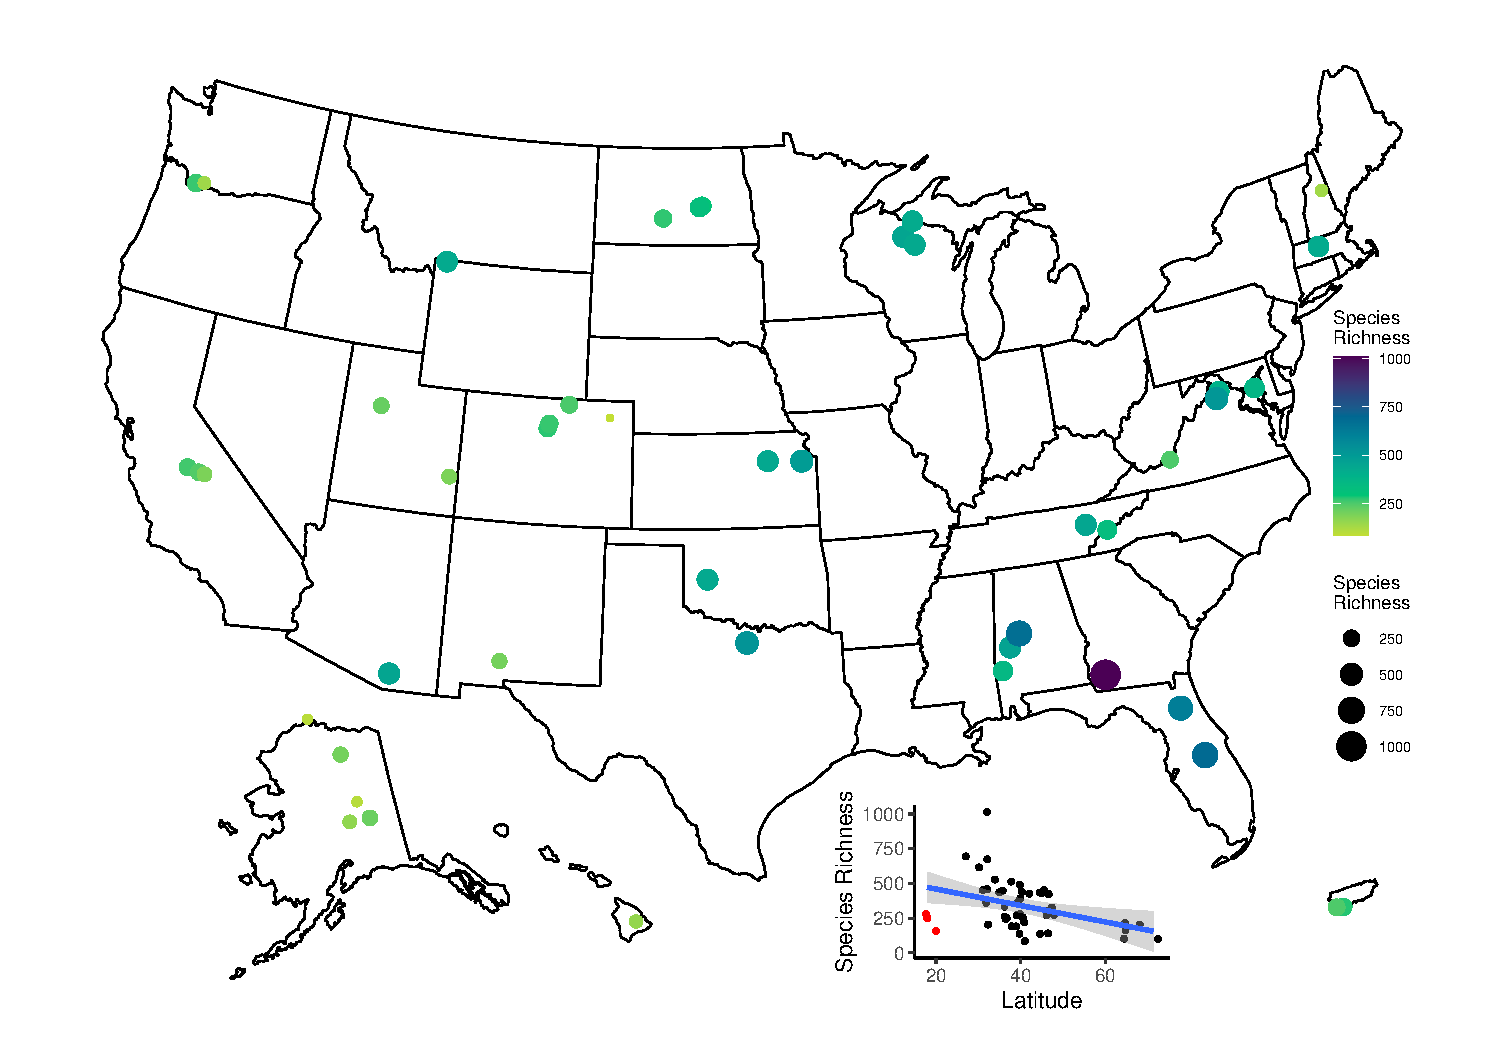
\includegraphics[width=0.95\linewidth]{/Users/dli/Github/neonDivData/manuscript/figures/p_plant} 

}

\caption{Plant species richness mapped across NEON terrestrial sites. The inset scatterplot shows latitude on the x-axis and species richness on the y-axis, with red points representing sites in Puerto Rico and Hawaii. Alaska, Hawaii, and Puerto Rico were rearranged to save space.}\label{fig:Fig2Map}
\end{figure}

In addition to allowing for quick exploration of macroecological patterns of diversity, the data products presented in this paper also enable investigation of effects of taxonomic resolution on diversity indices since taxonomic information is preserved for observations under family level for all taxonomic groups. The degree of taxonomic resolution varies for NEON taxa depending on the diversity of the group and the level of taxonomic expertise needed to identify an organism to the species level, with more diverse groups having greater uncertainty. Beetles are one of the most diverse groups of organisms on Earth and wide-ranging geographically, making them ideal bioindicators of environmental change (\protect\hyperlink{ref-rainio2003ground}{Rainio and Niemelä 2003}). To illustrate how the use of the beetle data product presented in this paper enables NEON data users to easily explore the effects of taxonomic resolution on community-level taxonomic diversity metrics, we calculated Jost diversity indices (\protect\hyperlink{ref-jost2006entropy}{Jost 2006}) for beetles at the Oak Ridge National Laboratory (ORNL) NEON site for data subsetted at the genus, species, and subspecies level. Jost indices are essentially Hill Numbers quantifying species diversity that vary in how abundance is weighted with a parameter q. Higher values of q give lower weights to low-abundance species with q = 0 being equivalent to species richness and q = 1 representing the effective number of species given by the Shannon entropy. These indices are plotted as rarefaction curves, which assess the sampling efficacy. When rarefaction curves asymptote they suggest that additional sampling will not capture additional taxa. Statistical methods presented by \protect\hyperlink{ref-chao2014rarefaction}{Chao et al.} (\protect\hyperlink{ref-chao2014rarefaction}{2014}) provide estimates of sampling efficacy beyond the observed data (i.e., extrapolated values shown by dashed lines in Fig. \ref{fig:Fig3Curve}). For the ORNL beetle data, Jost indices calculated with higher values of q (i.e., q \textgreater{} 0) indicate sampling has reached an asymptote in terms of capturing diversity regardless of taxonomic resolution (i.e., genus, species, subspecies). However, rarefaction curves for q = 0, which is equivalent to species richness do not asymptote, even with extrapolation. These plots suggest that if a researcher is interested in low abundance, rare species, then NEON beetle data streams at ORNL may need to mature with additional sample collections over time before confident inferences may be made, especially below the taxonomic resolution of genus.



\begin{figure}

{\centering 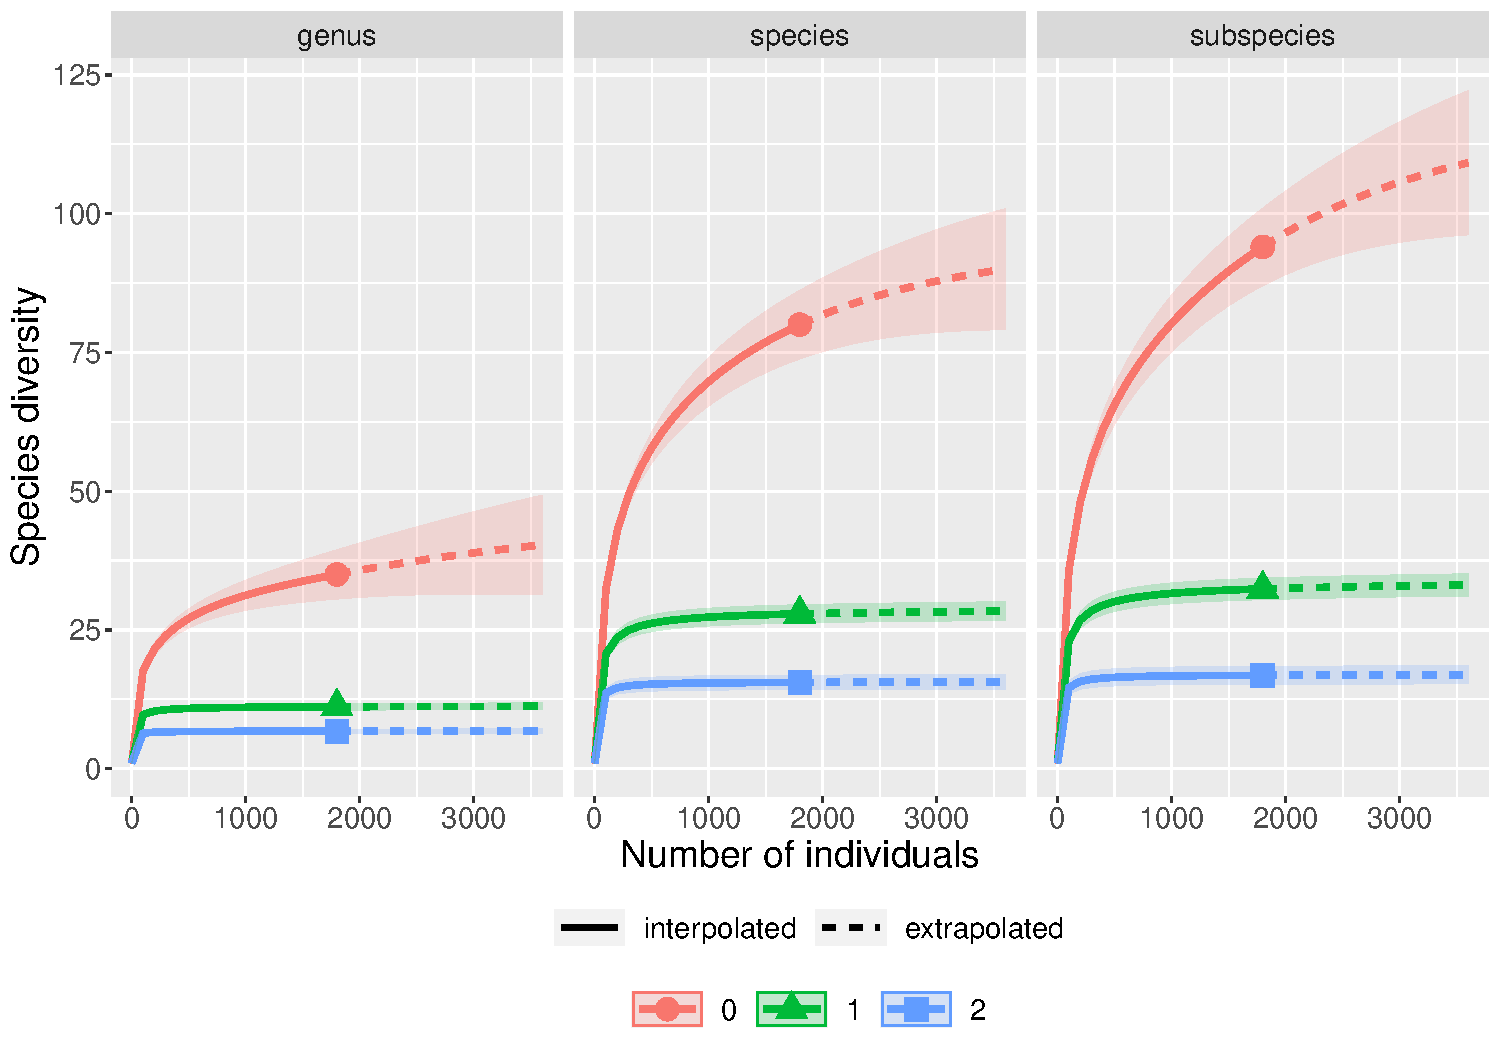
\includegraphics[width=0.95\linewidth]{/Users/dli/Github/neonDivData/manuscript/figures/beetle_rarefaction} 

}

\caption{Rarefaction of beetle abundance data from collections made at the Oak Ridge National Laboratory (ORNL) National Ecological Observatory Network (NEON) site from 2014-2020 generated using the iNEXT package in R (\protect\hyperlink{ref-hsieh2016inext}{Hsieh et al. 2016}) based on different levels of taxonomic resolution (i.e., genus, species, subspecies). Different colors indicate Jost Indices with differing values of q (\protect\hyperlink{ref-jost2006entropy}{Jost 2006}).}\label{fig:Fig3Curve}
\end{figure}

\hypertarget{discussion-or-how-to-maintain-and-update-tidy-neon-organismal-data}{%
\section{Discussion (or how to maintain and update tidy NEON organismal data)}\label{discussion-or-how-to-maintain-and-update-tidy-neon-organismal-data}}

NEON organismal data hold lots of potential to understand biodiversity change across space and time \protect\hyperlink{ref-jones2021synergies}{Jones et al.} (\protect\hyperlink{ref-jones2021synergies}{2021}). Multiple biodiversity research and education programs have used NEON data even before NEON became fully operational in May 2019 {[}CITATION{]}. With the expected large investment to maintain NEON over the next 30 years, NEON organismal data, alone or coupled with other major environmental datasets, will be invaluable to help us understand and track biodiversity change in an era of fast environmental change. NEON data are unique relative to data collected by other similar networks (e.g., LTER, CZO) because observation collection protocols are standardized across sites, enabling researchers to address macroscale questions in environmental science without having to synthesize disparate data sets that differ in collection methods (\protect\hyperlink{ref-jones2021synergies}{Jones et al. 2021}). Whereas the data collection protocols implemented by NEON staff are reproducible across space and time, the studies NEON data users perform after downloading NEON's open data will only be fully repeatable if the steps made to generate and analyze derived data sets are documented (\protect\hyperlink{ref-ellison2010repeatability}{Ellison 2010}). If such provenance is not curated for studies using NEON data, then 30 years from now we risk a situation where we find ourselves puzzling over inconclusive results from studies that use the same data. However, with careful provenance the gains in macroscale environmental knowledge have the potential to be transformative. By providing a standardized and easy-to-use data product of NEON organismal data, our effort here will significantly lower the barriers to use the NEON organismal data for biodiversity research by many current and future researchers and will ensure that studies using NEON data are reproducible.

Unlike NEON's organismal data, most long-term ecological community observations are made up of data where sampling protocols vary. The ecocomDP data design pattern was recently created to harmonize such community organismal observations to promote biodiversity synthesis efforts {[}O'Brien et al.~In review; \protect\hyperlink{ref-record2020novel}{Record et al.} (\protect\hyperlink{ref-record2020novel}{2020}){]}. The ecocomDP harmonized format is not bound by any research question (so long as it pertains to community level data), adds relevant metadata on the spatial and temporal scale of the derived data, and is amenable to different types of measurements (e.g., count, percent cover, biomass). The data package we present in this paper converts NEON organismal data to the ecocomDP format core tables (i.e., observation, taxon, location), so that NEON data will be more easily integrated with other community data sets, especially those available in the EDI repository (e.g., LTER, LTREB data). In the EDI repository, derived data sets are given DOIs, so that differences may be tracked from original to derived data sets. The data presented in this paper have their own DOIs that are discoverable through EDI and may be cited.

There are some important notes about the data product we provided. First, we did not check the taxonomy of all groups given that NEON already did its best to make sure that species identifications are correct. However, not every record was identified to species, with genus, family, or even order level species IDs in all groups. IDs above genus level may not be useful for most biodiversity projects. We thus decided to remove records with such IDs for groups that are relatively easier to identify (fish, plant, small mammals) or have very few taxon IDs that are above genus level (mosquito). However, for groups that are hard to identify (algae, beetle, bird, macroinvertebrate, tick, and tick pathogen), we decided to keep all records no matter what level of taxon IDs they have. Such information can be useful if we are interested in questions such as species-to-genus ratio or species rarefaction curves at different taxonomic levels (e.g., Fig. \ref{fig:Fig3Curve}). Users thus need to think carefully about which level of taxon IDs they need for their research. Second, we kept records without any observed species/individuals in some taxonomic groups (beetle, bird, small mammal). Such empty records still provide information about sampling efforts, which can be critical for some projects to control for. For example, if two sites both have the same number of small mammals during the same time period, however, one site has many more empty records (traps), then we can infer that the abundances of small mammals are lower than the other side. If such information is not needed in a project, then we can simply remove them. For algae and birds, we added standardized measurements as density and number of fish caught per hour, respectively, in the data product. Third, there are other organismal groups (Aquatic Microbes and Aquatic Plants; soil microbes were covered in Qin et al.~in this issue) not included in this study given the complexity of microbial data.

All codes that conducted the Data Wrangling Decisions were available online (Github and Zenodo, URL HERE). Therefore, users can easily reproduce the standardized data product, modify the code if they need to make different decisions during the data wrangling process, and correct any mistakes of our code by submitting a pull request to our repository. It is also easy to update the standardized data product when new data is uploaded by NEON to their data portal because the whole data wrangling workflow was automated. In fact, our Github repository is scheduled to run the whole workflow every year.

If researchers wish to generate their own derived organismal data sets from NEON data with slightly different decisions than the ones outlined in this paper, we recommend that they use the ecocomDP framework, upload the data to the EDI repository, and cite their data with the discoverable DOI given to them by EDI. Note that ecocomDP data design package was intended for community ecology analyses, so it will not handle individual data, such as those required for demographic analyses, well. A promising package for demographic analyses of NEON data is popler (\protect\hyperlink{ref-compagnoni2020popler}{Compagnoni et al. 2020}). The notion of different data packages for different levels of biological organization and different types of data raises the question of whether there are other data design packages that the NEON user community should adopt at the inception of the observatory. As the observatory moves forward, this is an important discussion to be had by the NEON user community and NEON technical working groups to promote synthesis of NEON data with data from other efforts (e.g., LTER, CZO, Ameriflux, the International LTER, National Phenology Network, Long Term Agricultural Research Network). It will also be important moving forward to make sure that funding for the maintenance of repositories, such as EDI, remains to prevent the loss of archived derived data sets.

The derived data products presented here collectively represent hundreds of hours of work by members of our team - a group that met at the NEON Science Summit in 2019 in Boulder, Colorado consisting of researchers and NEON science staff. Just as it is helpful when working with a dataset to either have collected the data or be in close correspondence with the person who collected the data, coming to many of these Data Wrangling Decisions benefited greatly from conversations with NEON science staff and the NEON user community. Future opportunities that encourage collaborations between NEON science staff and the NEON user community will be essential to achieve the full potential of the observatory in terms of transformative scientific discoveries.

\hypertarget{conclusion}{%
\section{Conclusion}\label{conclusion}}

Macrosystems ecology is at the start of an exciting new chapter with the decades long awaited buildout of NEON completed and standardized data streams from all sites in the observatory becoming publicly available online. As the research community embarks on discovering new scientific insights from NEON data, it is important that we strive to make our analyses and all derived data as reproducible as possible to ensure that connections across studies will be possible. Harmonized data sets will help in this endeavour because they naturally promote the collection of provenance as data are collated into derived products (O'Brien et al.~In review, \protect\hyperlink{ref-reichman2011challenges}{Reichman et al. 2011}). Harmonized data also make synthesis easier because efforts to clean and format data leading up to analyses do not have to be repeatedly performed by individual researchers (O' Brien et al.~In review). The derived data products presented here in the ecocomDP format illustrate a potential path forward in achieving a reproducible framework for data derived from NEON organismal data for community ecology analyses. \emph{Highlight value of collaboration between NEON user community and NEON staff for advancing NEON enabled science.}

\hypertarget{reference}{%
\section*{Reference}\label{reference}}
\addcontentsline{toc}{section}{Reference}

\hypertarget{refs}{}
\begin{CSLReferences}{1}{0}
\leavevmode\hypertarget{ref-baker1997environmental}{}%
Baker, J. R., D. V. Peck, and D. W. Sutton. 1997. Environmental monitoring and assessment program surface waters: Field operations manual for lakes. US Environmental Protection Agency, Washington.

\leavevmode\hypertarget{ref-balch2019neon}{}%
Balch, J. K., R. Nagy, and B. S. Halpern. 2019. NEON is seeding the next revolution in ecology. Frontiers in Ecology and the Environment 18.

\leavevmode\hypertarget{ref-barnett2019plant}{}%
Barnett, D. T., P. B. Adler, B. R. Chemel, P. A. Duffy, B. J. Enquist, J. B. Grace, S. Harrison, R. K. Peet, D. S. Schimel, T. J. Stohlgren, and others. 2019. The plant diversity sampling design for the national ecological observatory network. Ecosphere 10:e02603.

\leavevmode\hypertarget{ref-bechtold2005enhanced}{}%
Bechtold, W. A., and P. L. Patterson. 2005. The enhanced forest inventory and analysis program--national sampling design and estimation procedures. USDA Forest Service, Southern Research Station.

\leavevmode\hypertarget{ref-beck2014spatial}{}%
Beck, J., M. Böller, A. Erhardt, and W. Schwanghart. 2014. Spatial bias in the GBIF database and its effect on modeling species' geographic distributions. Ecological Informatics 19:10--15.

\leavevmode\hypertarget{ref-blowes2019geography}{}%
Blowes, S. A., S. R. Supp, L. H. Antão, A. Bates, H. Bruelheide, J. M. Chase, F. Moyes, A. Magurran, B. McGill, I. H. Myers-Smith, and others. 2019. The geography of biodiversity change in marine and terrestrial assemblages. Science 366:339--345.

\leavevmode\hypertarget{ref-brown2004toward}{}%
Brown, J. H., J. F. Gillooly, A. P. Allen, V. M. Savage, and G. B. West. 2004. Toward a metabolic theory of ecology. Ecology 85:1771--1789.

\leavevmode\hypertarget{ref-chao2014rarefaction}{}%
Chao, A., N. J. Gotelli, T. Hsieh, E. L. Sander, K. Ma, R. K. Colwell, and A. M. Ellison. 2014. Rarefaction and extrapolation with hill numbers: A framework for sampling and estimation in species diversity studies. Ecological monographs 84:45--67.

\leavevmode\hypertarget{ref-compagnoni2020popler}{}%
Compagnoni, A., A. J. Bibian, B. M. Ochocki, S. Levin, K. Zhu, and T. E. Miller. 2020. Popler: An r package for extraction and synthesis of population time series from the long-term ecological research (LTER) network. Methods in Ecology and Evolution 11:258--264.

\leavevmode\hypertarget{ref-curtis1959vegetation}{}%
Curtis, J. T. 1959. The vegetation of wisconsin: An ordination of plant communities. University of Wisconsin Pres.

\leavevmode\hypertarget{ref-egli2020taxonomic}{}%
Egli, L., K. E. LeVan, and T. T. Work. 2020. Taxonomic error rates affect interpretations of a national-scale ground beetle monitoring program at national ecological observatory network. Ecosphere 11:e03035.

\leavevmode\hypertarget{ref-ellison2010repeatability}{}%
Ellison, A. M. 2010. Repeatability and transparency in ecological research. Ecology 91:2536--2539.

\leavevmode\hypertarget{ref-farley2018situating}{}%
Farley, S. S., A. Dawson, S. J. Goring, and J. W. Williams. 2018. Situating ecology as a big-data science: Current advances, challenges, and solutions. BioScience 68:563--576.

\leavevmode\hypertarget{ref-fischer1960latitudinal}{}%
Fischer, A. G. 1960. Latitudinal variations in organic diversity. Evolution 14:64--81.

\leavevmode\hypertarget{ref-g2019remote}{}%
G Pricope, N., K. L Mapes, and K. D Woodward. 2019. Remote sensing of human--environment interactions in global change research: A review of advances, challenges and future directions. Remote Sensing 11:2783.

\leavevmode\hypertarget{ref-geldmann2016determines}{}%
Geldmann, J., J. Heilmann-Clausen, T. E. Holm, I. Levinsky, B. Markussen, K. Olsen, C. Rahbek, and A. P. Tøttrup. 2016. What determines spatial bias in citizen science? Exploring four recording schemes with different proficiency requirements. Diversity and Distributions 22:1139--1149.

\leavevmode\hypertarget{ref-gurevitch1999statistical}{}%
Gurevitch, J., and L. V. Hedges. 1999. Statistical issues in ecological meta-analyses. Ecology 80:1142--1149.

\leavevmode\hypertarget{ref-hampton2013big}{}%
Hampton, S. E., C. A. Strasser, J. J. Tewksbury, W. K. Gram, A. E. Budden, A. L. Batcheller, C. S. Duke, and J. H. Porter. 2013. Big data and the future of ecology. Frontiers in Ecology and the Environment 11:156--162.

\leavevmode\hypertarget{ref-hillebrand2004generality}{}%
Hillebrand, H. 2004. On the generality of the latitudinal diversity gradient. The American Naturalist 163:192--211.

\leavevmode\hypertarget{ref-hoekman2017design}{}%
Hoekman, D., K. E. LeVan, C. Gibson, G. E. Ball, R. A. Browne, R. L. Davidson, T. L. Erwin, C. B. Knisley, J. R. LaBonte, J. Lundgren, and others. 2017. Design for ground beetle abundance and diversity sampling within the national ecological observatory network. Ecosphere 8:e01744.

\leavevmode\hypertarget{ref-hoekman2016design}{}%
Hoekman, D., Y. P. Springer, C. Barker, R. Barrera, M. Blackmore, W. Bradshaw, D. H. Foley, H. S. Ginsberg, M. Hayden, C. Holzapfel, and others. 2016. Design for mosquito abundance, diversity, and phenology sampling within the national ecological observatory network. Ecosphere 7:e01320.

\leavevmode\hypertarget{ref-hsieh2016inext}{}%
Hsieh, T., K. Ma, and A. Chao. 2016. iNEXT: An r package for rarefaction and extrapolation of species diversity (h ill numbers). Methods in Ecology and Evolution 7:1451--1456.

\leavevmode\hypertarget{ref-hubbell2001unified}{}%
Hubbell, S. P. 2001. The unified neutral theory of biodiversity and biogeography (MPB-32). Princeton University Press.

\leavevmode\hypertarget{ref-hutchinson1959homage}{}%
Hutchinson, G. E. 1959. Homage to santa rosalia or why are there so many kinds of animals? The American Naturalist 93:145--159.

\leavevmode\hypertarget{ref-jones2021synergies}{}%
Jones, J., P. Groffman, J. Blair, F. Davis, H. Dugan, E. Euskirchen, S. Frey, T. Harms, E. Hinckley, M. Kosmala, and others. 2021. Synergies among environmental science research and monitoringnetworks: A research agenda. Earth's Future:e2020EF001631.

\leavevmode\hypertarget{ref-jost2006entropy}{}%
Jost, L. 2006. Entropy and diversity. Oikos 113:363--375.

\leavevmode\hypertarget{ref-keller2008continental}{}%
Keller, M., D. S. Schimel, W. W. Hargrove, and F. M. Hoffman. 2008. A continental strategy for the national ecological observatory network. The Ecological Society of America: 282-284.

\leavevmode\hypertarget{ref-koricheva2014uses}{}%
Koricheva, J., and J. Gurevitch. 2014. Uses and misuses of meta-analysis in plant ecology. Journal of Ecology 102:828--844.

\leavevmode\hypertarget{ref-li2020changes}{}%
Li, D., J. D. Olden, J. L. Lockwood, S. Record, M. L. McKinney, and B. Baiser. 2020. Changes in taxonomic and phylogenetic diversity in the anthropocene. Proceedings of the Royal Society B 287:20200777.

\leavevmode\hypertarget{ref-linnaeus1758systema}{}%
Linnaeus, C. 1758. Systema naturae. Stockholm Laurentii Salvii.

\leavevmode\hypertarget{ref-macarthur1967theory}{}%
MacArthur, R. H., and E. O. Wilson. 1967. The theory of island biogeography. Princeton university press.

\leavevmode\hypertarget{ref-martin2012mapping}{}%
Martin, L. J., B. Blossey, and E. Ellis. 2012. Mapping where ecologists work: Biases in the global distribution of terrestrial ecological observations. Frontiers in Ecology and the Environment 10:195--201.

\leavevmode\hypertarget{ref-midgley2005global}{}%
Midgley, G. F., and W. Thuiller. 2005. Global environmental change and the uncertain fate of biodiversity. The New Phytologist 167:638--641.

\leavevmode\hypertarget{ref-moulton2002revised}{}%
Moulton II, S. R., J. G. Kennen, R. M. Goldstein, and J. A. Hambrook. 2002. Revised protocols for sampling algal, invertebrate, and fish communities as part of the national water-quality assessment program. Geological Survey (US).

\leavevmode\hypertarget{ref-nakagawa2012methodological}{}%
Nakagawa, S., and E. S. Santos. 2012. Methodological issues and advances in biological meta-analysis. Evolutionary Ecology 26:1253--1274.

\leavevmode\hypertarget{ref-palumbo2017building}{}%
Palumbo, I., R. A. Rose, R. M. Headley, J. Nackoney, A. Vodacek, and M. Wegmann. 2017. Building capacity in remote sensing for conservation: Present and future challenges. Remote Sensing in Ecology and Conservation 3:21--29.

\leavevmode\hypertarget{ref-pavlacky2017statistically}{}%
Pavlacky Jr, D. C., P. M. Lukacs, J. A. Blakesley, R. C. Skorkowsky, D. S. Klute, B. A. Hahn, V. J. Dreitz, T. L. George, and D. J. Hanni. 2017. A statistically rigorous sampling design to integrate avian monitoring and management within bird conservation regions. PloS one 12:e0185924.

\leavevmode\hypertarget{ref-peck2006environmental}{}%
Peck, D. V., Herlihy, A. T., Hill, B. H., Hughes, R. M., Kaufmann, P. R., Klemm, D. J., Lazorchak, J. M., McCormick, F. H., Peterson, S. A., Ringold, P. L., Magee, T., and M. R. and Cappaert. 2006. Environmental monitoring and assessment program --- surface waters: Western pilot study field operations manual for wadeable streams. US Environmental Protection Agency, Washington.

\leavevmode\hypertarget{ref-pritt2017proposal}{}%
Pritt, B. S., M. E. Allerdice, L. M. Sloan, C. D. Paddock, U. G. Munderloh, Y. Rikihisa, T. Tajima, S. M. Paskewitz, D. F. Neitzel, D. K. H. Johnson, and others. 2017. Proposal to reclassify ehrlichia muris as ehrlichia muris subsp. Muris subsp. Nov. And description of ehrlichia muris subsp. Eauclairensis subsp. Nov., A newly recognized tick-borne pathogen of humans. International journal of systematic and evolutionary microbiology 67:2121.

\leavevmode\hypertarget{ref-rainio2003ground}{}%
Rainio, J., and J. Niemelä. 2003. Ground beetles (coleoptera: Carabidae) as bioindicators. Biodiversity \& Conservation 12:487--506.

\leavevmode\hypertarget{ref-ralph1993handbook}{}%
Ralph, C. J. 1993. Handbook of field methods for monitoring landbirds. Pacific Southwest Research Station.

\leavevmode\hypertarget{ref-read2018among}{}%
Read, Q. D., J. M. Grady, P. L. Zarnetske, S. Record, B. Baiser, J. Belmaker, M.-N. Tuanmu, A. Strecker, L. Beaudrot, and K. M. Thibault. 2018. Among-species overlap in rodent body size distributions predicts species richness along a temperature gradient. Ecography 41:1718--1727.

\leavevmode\hypertarget{ref-record2020novel}{}%
Record, S., N. M. Voelker, P. L. Zarnetske, N. I. Wisnoski, J. D. Tonkin, C. Swan, L. Marazzi, N. Lany, T. Lamy, A. Compagnoni, and others. 2020. Novel insights to be gained from applying metacommunity theory to long-term, spatially replicated biodiversity data. Frontiers in Ecology and Evolution 8:479.

\leavevmode\hypertarget{ref-reichman2011challenges}{}%
Reichman, O. J., M. B. Jones, and M. P. Schildhauer. 2011. Challenges and opportunities of open data in ecology. Science 331:703--705.

\leavevmode\hypertarget{ref-rudenko2011updates}{}%
Rudenko, N., M. Golovchenko, L. Grubhoffer, and J. H. Oliver Jr. 2011. Updates on borrelia burgdorferi sensu lato complex with respect to public health. Ticks and tick-borne diseases 2:123--128.

\leavevmode\hypertarget{ref-sauer2017first}{}%
Sauer, J. R., K. L. Pardieck, D. J. Ziolkowski Jr, A. C. Smith, M.-A. R. Hudson, V. Rodriguez, H. Berlanga, D. K. Niven, and W. A. Link. 2017. The first 50 years of the north american breeding bird survey. The Condor: Ornithological Applications 119:576--593.

\leavevmode\hypertarget{ref-thorpe2016introduction}{}%
Thorpe, A. S., D. T. Barnett, S. C. Elmendorf, E.-L. S. Hinckley, D. Hoekman, K. D. Jones, K. E. LeVan, C. L. Meier, L. F. Stanish, and K. M. Thibault. 2016. Introduction to the sampling designs of the n ational e cological o bservatory n etwork t errestrial o bservation s ystem. Ecosphere 7:e01627.

\leavevmode\hypertarget{ref-vellend2013global}{}%
Vellend, M., L. Baeten, I. H. Myers-Smith, S. C. Elmendorf, R. Beauséjour, C. D. Brown, P. De Frenne, K. Verheyen, and S. Wipf. 2013. Global meta-analysis reveals no net change in local-scale plant biodiversity over time. Proceedings of the National Academy of Sciences 110:19456--19459.

\leavevmode\hypertarget{ref-wilkinson2016fair}{}%
Wilkinson, M. D., M. Dumontier, Ij. J. Aalbersberg, G. Appleton, M. Axton, A. Baak, N. Blomberg, J.-W. Boiten, L. B. da Silva Santos, P. E. Bourne, and others. 2016. The FAIR guiding principles for scientific data management and stewardship. Scientific data 3:1--9.

\leavevmode\hypertarget{ref-worm2018theory}{}%
Worm, B., and D. P. Tittensor. 2018. A theory of global biodiversity (MPB-60). Princeton University Press.

\end{CSLReferences}

\end{document}
